%\documentclass{unmeereport}
%\documentclass[final]{eeceTR} - using the final option changes layout
\documentclass[botnum, nobox]{unmeethesis}

% TODO Numbering starts on first chapter. Should be roman numerals before that, not required.

\usepackage{multirow}  % for the table
\usepackage{color, colortbl}
\definecolor{LightGray}{gray}{.9} % for table rows
\usepackage{relsize}
\usepackage{graphicx}

\begin{document}

\frontmatter

% Uncomment the next command if you see weird paragraph spacing:
% That is, if you see paragraphs float with lots of white space
% in between them:
% \setlength{\parskip}{0.30cm}


\title{Mesh Addition Based on the Depth Image (MABDI)}

\author{Lucas E. Chavez}

\degreesubject{M.S., Mechanical Engineering}

\degree{Master of Science \\ Mechanical Engineering}

\documenttype{Thesis}

\previousdegrees{B.S., Mechanical Engineering \\
New Mexico Institute of Mining and Technology, 2009}

\date{December, 2016}

\maketitle

% \begin{dedication}
%    To my parents, Albert II and Gladys, for their support,
%    encouragement and the Corvette they're giving me for graduation. \\[3ex]
%    ``A bird in hand is worth two in the bush''
%          -- Anonymous
% \end{dedication}

\begin{acknowledgments}
   \vspace{1.1in}
   This work was support in part by Sandia National Laboratories under Purchase
   Order: 1179196 and  NSF grant OISE \#1131305.
\end{acknowledgments}

\maketitleabstract %(required even though there's no abstract title anymore)

\begin{abstract}
  Many robotic applications, especially those whose goal is to aid or assist
  through human-robot interaction, utilize a rich map of the world for reasoning
  tasks such as collision detection, path planning, or object recognition. Such
  map, and the method used to produce it, must take into consideration
  real-world constraints. Most mesh-based mapping algorithms resemble a ``black
  box'' and do not provide a mechanism to close the loop and make decisions
  about the incoming information. MABDI leverages the global mesh by finding the
  difference between what we expect to see and what we are actually seeing, and
  using this to classify the incoming measurements as novel or not. This allows
  the surface reconstruction method to be run only on data that has not yet been
  represented in the global mesh. The result is an algorithm that becomes
  computationally inexpensive once the environment is known, but can also react
  to new objects.
\clearpage %(required for 1-page abstract)
\end{abstract}

\tableofcontents
\pagebreak

\mainmatter


\chapter{Introduction} \label{chapter:introduction}
\section{Overview}

% Overview
% * applications need a map
% * methods have been evolving, fueled by new sensors. In particular RGB-D
%   RGB-D Sensors
%   * Specs of RGB-D sensors, create lots of data
%   * Mapping methods must be able to handle this data
%   Maps
%   * slam problem, we are concerned with mapping
%   * types of maps, we are concerned with rich types
%   * list of constraints: supported, computation, memory
%   * discussion of why mesh
% Goal
% * Create a system that can intelligently make decisions about sensor data
%   * Using tools already developed for mesh
%   * Computationally feasible
%   * Leverage information that we already know
% Contribution
% * Discussion of difference with "black box" methods

% Overview
% * applications need a map
% * methods have been evolving, fueled by new sensors
% * slam problem, we are concerned with mapping
% * types of maps, we are concerned with rich types
% * list of constraints: supported, computation, memory
% * discussion of why mesh
% Contribution
% * Discussion of difference with "black box" methods

Many robotic applications, especially those that involve human-robot
interaction, often require a rich representation of the environment in order to
perform such behavior as path planning and obstacle avoidance. In general, a
rich representation, or map, is useful for providing situational awareness to an
autonomous agent. A map is also important for applications such as teleoperation
\cite{Kadous2006}.

In robotics, map building in an unknown environment is referred to as the
Simultaneous Localization and Mapping (SLAM) problem \cite{Thrun2002}. This
label describes the fact that a methodology which solves the SLAM problem must
simultaneously locate the robot in the environment as well as map the
environment. The focus of this work is the mapping aspect of the SLAM problem.
Fig. \ref{fig:goal} gives a visualization of the goal.

\begin{figure}[h]%[thpb]
\centering
  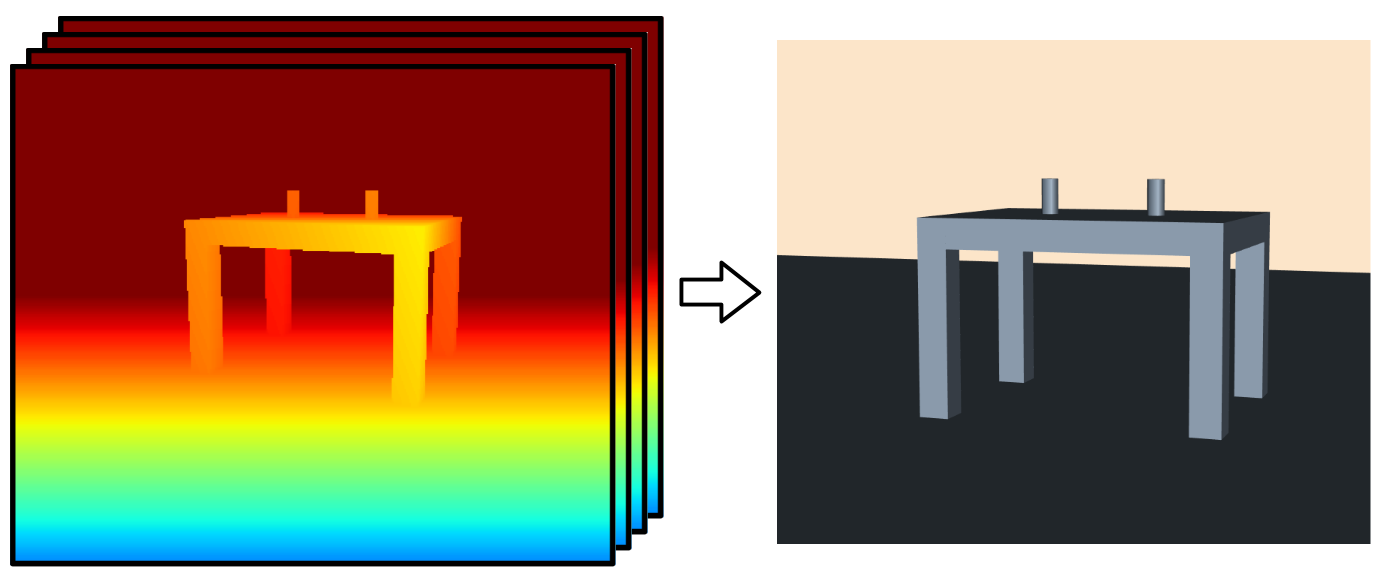
\includegraphics[width=.75\textwidth]{figures/diagram_goal.png}
  \caption{Goal is to create a map from depth images.}
  \label{fig:goal}
\end{figure}

The methodology to build a map is a continuously evolving subject in the field
of robotics and computer graphics. Well known works of map building methods
began to be seen around 1987 \cite{Lorensen1987}. Since then, the methods and
the representations themselves have continued to evolve at an impressive rate.
Growth in this field of research has been fueled by continuous advances in
computing and sensing technologies. Over the years, sensors have continued to
generate measurements at higher rates, higher resolution, and lower cost. RGB-D
sensors are a new category of sensor that have recently gained extensive
popularity in the robotics community due to their affordability and ability to
generate a rich amount of data.

\subsection{RGB-D Sensors}

The popularity of RGB-D sensors began with the release and commercialization of
the Kinect\texttrademark ~ by Microsoft. The arrival of the Kinect brought with
it an inexpensive depth sensor that uses an active range system to generate a
depth map of a given environment \cite{freedman2012depth}. The Kinect and similar
sensors, have come to be called RGB-D sensors. This class of sensors provide
images which include both visual (RGB) and depth (D) values.
Several works have taken advantage of this sensor technology in scenarios such
as environmental mapping \cite{henry2012rgb}, 3D reconstruction
\cite{Newcombe2011a}, gesture recognition \cite{Xia2011}, and altitude control of
aerial vehicles \cite{Stowers2011}.

RGB-D sensors generally provide data at 30 frames per second and 640$\times$480
resolution. Consequently, methods that use RGB-D data must handle over 9 million
pixel values per second, if only using the depth information (D), and over 18
million if using both color (RGB) and depth (D). The magnitude of the amount of
data output from RGB-D sensors creates the need for mapping methods that are
computationally inexpensive and also influences the type of data structure used
to store the map.

\subsection{Maps}

There are different types of data structures that can define a map. All types
have both intrinsic characteristics that impact the algorithms that generate
them and constraints that must be considered for real-world applications. In
addition, we are concerned with rich representation types, in contrast to sparse
representation types \cite{Dissanayake2001}, because rich types have the most
use in applications such as human-robot interaction.

\begin{table}[h]
  \caption{Comparison of constraints for different map types.}
  \label{tab:rep}
  \begin{footnotesize}
  \begin{center}
    \begin{tabular}{|l|c|c|c|c|c|}
    \hline
    \multirow{2}{*}{}   & Supported & Computationally & Low Memory  \\
                        &           & Inexpensive     & Requirement \\\hline
    Point Clouds		    & x         & x               & -           \\
    Surfels             & -         & x               & x           \\
    Implicit Functions 	& x         & -               & -           \\
    Mesh	 	            & x         & x               & x           \\
    \hline
    \end{tabular}
  \end{center}
  \end{footnotesize}
\end{table}

When considering which type of map is best for real-world applications, we must
consider the constraints imposed by each type:

\begin{itemize}
  \item Supported - Is there software, tools, research, algorithms, etc., for
  this type of map?
  \item Computationally Inexpensive - Can the algorithms run quickly on low cost
  computers (rather than specialized hardware)?
  \item Low Memory Requirement - Can the algorithms run on hardware with
  a standard amount of RAM?
\end{itemize}

Table \ref{tab:rep} compares the constraints of common map types. We can see, in
general a mesh type map satisfies real-world constraints. Additionally, meshes have
been used extensively by the gaming and graphics communities, and so benefits
from an incredible amount of continued research and advances in hardware such as
Graphics Processing Units (GPUs).

\section{Goal}

The goal of this work is to develop a mapping algorithm that can gracefully
utilize the amount of data output from an RGB-D sensor. Additionally, the
algorithm will make use of software tools and hardware that have been developed
for mesh data structures. The algorithm will be able to make intelligent
decisions using the data it receives based on the knowledge it has been building
about the environment. The decisions will be driven by the leveraging the
difference between what the algorithm is actually seeing and what it expects to
see. The decisions will be generated using computationally inexpensive computer
vision methods.

\section{Contribution}

Currently, one of the issues with mesh mapping techniques is they are generally
``black box'' methods. Meaning the data comes in from the sensor, those
measurements are turned into a mesh, and then that mesh is appended to a global
mesh. Fig. \ref{fig:pipeline} visualizes this common pipeline in black. The goal
of this work is to design an algorithm to close the loop (as visualized in red)
and allow the system to make decisions about the incoming data based on what it
already knows.

\begin{figure}[h]%[thpb]
\centering
  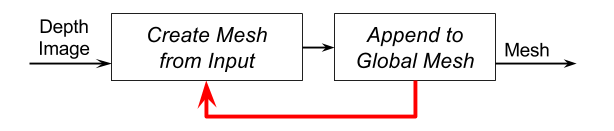
\includegraphics[width=.75\textwidth]{figures/diagram_general_pipeline.png}
  \caption{Common ``black box'' pipeline in black. The contribution of MABDI in red.}
  \label{fig:pipeline}
\end{figure}

% design goals of the system

\chapter{Related Works}	\label{chapter:related_works}

% Works related to MABDI are generally based on RGB-D sensors. This type of sensor has
% become very popular since the release of the Kinect from Microsoft, which
% was the first mass produced RGB-D sensor of its kind. RGB-D sensors are
% inexpensive and produce noisy 640x480 depth images at 30fps. The RGB-D
% sensor has excited the robotics community because this has been the first
% time that depth data has been so readily accessible from such an
% inexpensive sensor. Therefore, methodologies that use RGB-D data must be able to quickly
% deal with very high rates of information.
%
% Research and development of new mapping algorithms trend towards
% leveraging the information in the global map to make decisions about the
% incoming data. One can see parallels with how we as humans see the world. MABDI
% proposes do this in a computationally feasible way by simply using
% differencing and thresholding imaging methods.


A major problem in robotics has been and continues to be: How can we create the
``best'' representation of an unknown environment? There are two main
communities of researchers who been working on developing algorithms and methods
to answer precisely this question. They are the robotics community and the
computer graphics community, but each community has a slightly different
motivation for solving this problem. The robotics community is concerned with
developing a real-time solution for generating representations in large
environments. In the literature, large environments usually range in size from
multi-room office spaces to a few square miles on city streets. These
representations are used by both fully autonomous and teleoperated systems. The
common name which is used by the robotics community for this problem is
Simultaneous Localization and Mapping or SLAM. The name SLAM refers to the
problem of mapping and locating a robot in an unknown environment. Early methods
generated very sparse representations of the world, as time and sensor
technology progressed the representations became denser. A dense representation
is desired for any system that must have good situational awareness of its
environment. The computer graphics community is concerned with generating high
quality representations of small environments. In the literature, small
environments usually range in size from a cubic meter to room size. They
generally refer to the problem as surface reconstruction. These representations
are used by augmented reality, computer game object creation, 3D printing, and
other applications. In the following sections we will trace the development of
representation generating methods in both communities.

\section{SLAM}

The problem of SLAM has been a primary focus of the robotics community for
more than 25 years. A complete solution to the SLAM problem must be able to
generate a representation of an unknown environment and track the robot in
this new representation. In this body of literature the act of generating a
representation is referred to as mapping. A good overview of the problem
can be found in \cite{Durrant-Whyte2006} and \cite{Bailey2006}. Each
solution is designed to consider the goal application, type of sensor,
computational constraints, and memory limits. All these factors influence
the researcher's choice of which type of representation to use for the
mapping procedure. In 2002 Thrun wrote a famous survey \cite{Thrun2002} of
the SLAM literature which categorized existing algorithms on many traits
including the representation. The representation choice of prior work can
be roughly categorized into three types. The first type is characterized by
some sort of list of 2D or 3D points and are usually considered to be
sparse representations. Common names for these types are landmark locations
and point clouds. The second type is considered to be more volumetric
based and is often times considered to be a dense representation. Common
names for these types are occupancy grid and Truncated Signed Distance
Function (TSDF). The last type has the characteristic of being a surface
representation and is also considered to be a dense representation. Common
names for these types are surfels and mesh. In the following sections we
will trace the history of each of the three types of representation that are
seen in the SLAM literature.

\subsection{Point Locations}

One of the most well known and earliest solution to the SLAM problem, which
uses a point location representation, was proposed by Smith et al. in 1990
\cite{Smith1990}. The mathematical framework that he created was the origin
of a family of solutions based on the Extended Kalman Filter (EKF). The
representation he chose was simply a list of 2D landmark locations. Each
location was part of a state matrix which was estimated at every iteration.
A list of landmark locations was chosen because it allowed the method to
have a low computational cost and use a small amount of memory, important
factors in the days of early computing. There have been many improvements
to the family of SLAM solutions which generate a list of point locations
since Smith's work. One of the first practical implementations on a real
robot was done by Thrun in 1998 \cite{Thrun1998}. In this work the SLAM
problem was posed in an Expectation Maximization (EM) framework which is
similar to the EKF framework in that landmark locations are saved
in a state vector which is estimated at every iteration. In Thrun's work an
occupancy grid map is generated as a post processing step from sonar
measurements. The results showed that their representation could become
more accurate over time by using new observations to improve the current
estimate. This a highly desired ability of any representation generation
method. The next step was the ability of these methods to include a loop
closure procedure. A loop closure procedure was proposed by Gutmann in 1999
\cite{Gutmann1999}. The key ability of the method was it could recognize
when the robot was revisiting a prior location and adjust the entire
representation with the constraint that the two points must coincide. In
2001 Dissanayake et al. \cite{Dissanayake2001} derived three theorems to
theoretically prove the convergence of the SLAM problem. Their test
platform used a millimeter-wave radar mounted on a vehicle and generated a
list of 2D landmark locations. In 2001 Thrun et al. \cite{Thrun2001} cast
the SLAM problem using particle filter techniques. Their results generated
a 2D map and showed an increased robustness and lower computational cost
than prior methods. One of the key disadvantages of methods up to this
point was that complexity scaled quadratically with the number of landmark
locations. In 2002 Montemerlo et al. \cite{Montemerlo2002} created a SLAM
solution named FastSLAM, which was able to handle a much larger number of
landmarks. They showed results with maps containing more than 50,000
points. Then, SLAM solutions using point locations became much more
directed towards 3D.

Some of the first interesting works that represented the world as a list of 3D
point locations were done by Thrun et al. in 2000 \cite{Thrun2000}, Liu and
Emery in 2001 \cite{Liu2001}, and H\"{a}hnel et al. in 2003. In these works the
2D landmark locations and robot position were estimated using techniques from
Thrun's past work \cite{Thrun1998}. Once this had been done the 3D laser scan
data was simply appended to each estimated robot location. Then, a mesh was
created by post processing the 3D point cloud. Their works utilized the fact
that the laser collected the data in an incremental manner and simply connected
neighboring 3D points. Finally, the mesh was simplified by looking for large
planar sections and merging the corresponding mesh elements. One of the first
SLAM solutions which used a single camera to generate a list of 3D points was
done by Davison in 2003 \cite{Davison2003}. Here he used a single camera to
generate a very sparse list of 3D points. This method was limited to small
environments. Future advances allowed representations of larger environments. In
2003 Thrun et al. \cite{Thrun2003} created a SLAM procedure which did not rely
on having a structured environment and was applied to mapping large mines. In
2004 Howard et al. \cite{Howard2004} created a SLAM system based on a Segway
platform equipped with a 3D laser which could map areas of roughly 0.5 km on
each side. One of the results showed a map with approximately 8 million points.
In 2006 Cole and Newman \cite{Cole2006} continued work in large-scale SLAM by
increasing robustness and also generated maps with many 3D points using a laser
sensor. In 2007 Clemente et al. created a large-scale SLAM system that used a
single camera. The system had an advanced loop closing procedure based on visual
features and created large maps of 3D points. In 2001 Klein and Murray
\cite{Klein2007} developed a SLAM solution which used a single camera. The
uniqueness of their method was the algorithmic structure. Their SLAM solution
consisted of two separate processes: a tracking process and a map building
process. This algorithmic structure has become very common in many current SLAM
solutions because of the advances in pose estimation technology. Klein and
Murray were able to get very good results for a small environment and showed
Augmented Reality (AR) applications. Many of the future advances of SLAM
solutions, which generated 3D point sets, dealt with camera systems
\cite{Paz2008,Konolige2008,Strasdat2010} and improved speed and robustness. Most
current methods that produce a list of points use a relatively new type of
sensor named a RGB-D sensor. One good example is a work that was produced in
2011 by Engelhard et al. \cite{Engelhard2011}. In this work they used an
algorithm named the Iterative Closest Point (ICP) \cite{Rusinkiewicz} to align
point clouds coming from the RGB-D sensor into a large colored point cloud. The
resulting maps were visually impressive. However, the map could not be adapted
to new information and was not well suited for other applications, such as
obstacle avoidance. These limitations are inherent in maps that consist of lists
of points.

\subsection{Volumetric}

Many SLAM solutions generate a 2D volumetric representation of the world
because they are especially advantageous in dealing with noisy sensors. Two
of the first major works that generated a 2D volumetric representation
were done in 1998 by Yamauchi et al. \cite{Yamauchi1998} and Schultz et al.
\cite{Schultz1998}. These works generated a 2D occupancy grid, which is a
type of volumetric representation. Here the environment was divided into a
2D grid. Each square of the grid contained the probability that it was
occupied with an object. All squares would be updated iteratively based on
the current sensor readings. Occupancy grids, like any other
volumetric-based representation, are limited by the amount of available
memory. In 2002 Biswas et al. \cite{Biswas2002} extended occupancy grid
methods by allowing dynamic environments. This was done by looking at past
``snapshots'' of the map. In 2004 Eliazar and Parr \cite{Eliazar2004}
continued the advancement by decreasing computational cost and implemented
a loop closure method.

There have been a few impressive SLAM solutions that generate a 3D volumetric
representation. There are three major works that generated a result very similar
to a 3D occupancy grid, which was saved as in a octree data structure
\cite{Magnusson2007,Nuchter2007,Huang2011,Endres2012}. Each work had a slightly
different name and procedure for generating the representation, but in general
the representations divided the environment into cubes and had a scalar value
representing the belief of a surface being there. Octrees were used to save
memory by only having a fine resolution of cubes at places where there was a
surface. There are many advantages to a 3D occupancy grid representation. The
representation is well suited for obstacle avoidance and path planning
applications. Also, the representation is very adaptable to new information. The
major disadvantage is that the representation can not be visualized immediately.
In order to render, an image must be generated at each desired viewpoint by ray
tracing the volume. This can be a problem when using such method for
applications such as teleoperation due to the computational cost of rendering.
The current state of the art for generating a volumetric representation was done
by Newcombe et al. in 2011 \cite{Newcombe2011a}. Their system used a RGB-D
sensor and generated a 3D voxelized grid Truncated Signed Distance Function
(TSDF) of the environment. For this type of representation each cube contains
the value of the distance to the nearest surface. The sign of the value is based
on which side of the surface the cube is relative to the sensor. This work has
been the most capable at dealing with extremely noisy data and dynamic scenes.
However, due to memory constraints the method can only represent environments
that are about the size of a 4m cube. Also, it must be ray traced in order to be
visualized.

\subsection{Surface}

One of the first major works that created a surface representation of the
environment in real-time was done by Martin and Thrun in 2002 \cite{Martin2002}.
Their method utilized an EM framework to fit plane models to 3D point cloud
data. Polygon mesh elements were then easily assigned to each plane. The main
drive behind this work was to generate a map of the environment that uses a
small amount of memory. Their  method worked well for structured environments.
One of the major limitations of their method, and other methods that only mesh
large planar sections, is that the representation will only consist of planar
sections and not capture the fine detail of the environment. In 2004 Viejo and
Cazorla \cite{Viejo2004} developed a methodology for generating a mesh that can
contain more information of the environment than large planar sections. Due to
this ability, they termed their method to be ``unconstrained.'' Essentially
their method was based on a 3D Delaunay triangulation algorithm. Giesen surveyed
Delaunay triangulation methods in \cite{Giesen2004}. Viejo and Cazorla were not
able to obtain real-time results and, in fact, it has been seen that it is
extremely difficult to run a 3D Delaunay triangulation in real time because of
the numerous distance calculations required. One of the next major advances came
from Weingarten and Siegwart in 2006 \cite{Weingarten2006}. Their work also
created a mesh that was only capable of capturing large planar surfaces.
However, they showed increased robustness. In 2007 Pollefeys et al.
\cite{Akbarzadeh2006,Pollefeys2007} developed a large urban mapping system
consisting of a vehicle and eight camera systems. The processing was carried out
by multiple CPUs and optimized for speed with Graphics Processing Unit (GPU)
calculations. In their work they used the camera systems to generate an initial
set of depth maps. This set was then reduced using their depth map fusion
method. The method combined multiple depth maps to reject erroneous depth
estimates and remove redundancy from the data, resulting in a reduced set of
depth maps that was more accurate than the initial set of depth maps. The
reduced set was then used by a triangulation procedure to create a mesh of the
environment. The mesh generation procedure was based on a work from 2002 by
Pajarola et al. \cite{Pajarola2002}. This method defines a mesh in the depth
image. It starts from a very coarse mesh and continues to refine in areas of the
depth image based on a confidence criteria. In the work of Weingarten and
Siegwart, these meshes that are defined for each fused depth image are then
checked for overlaps and duplicates are removed to make a single large mesh. One
of the major drawbacks of this approach is that the output mesh can not be
adapted by measurements that come from revisited parts of the scene. Another
major advancement came in 2008 from Poppinga et al. \cite{Poppinga2008}. In this
work they used a Time of Flight (ToF) camera to generate a mesh representation
of the large planar structures in the environment. Here they also develop a
procedure to determine a mesh in a depth image. They leverage the structure of
the depth image to make the method computationally inexpensive. In their work
they simply append the meshes that are created from each depth image into a
global coordinate system. They obtain very good results from a simple method.
However, the method is not adaptive to new information. Also, a mesh is created
for each depth image instead of updating and maintaining a global mesh. A major
advancement came from work done by Newcombe and Davison in 2010
\cite{Newcombe2010}. In this work they designed a method to create a mesh
reconstruction from a single video camera. Their method used Structure From
Motion (SFM) to obtain a sparse point cloud of the scene. Then an implicit
function was fit to the point cloud using the methodology of Ohtake et al.
\cite{Ohtake2003}. A bundle of depth maps is then selected. From the bundle a
single reference depth image is selected and a ``base'' model is constructed by
sampling the implicit surface for vertices in the reference frame. The
neighboring frames are used to better the ``base'' model and create a more
accurate mesh. Each reference frame has its own mesh and all the meshes are put
into a global coordinate system. Duplications are then detected and removed.
Again, the representation is not adaptive to new information. In 2010
St\"{u}hmer et al. \cite{Stuhmer2010} generated very accurate depth maps from
several color images in real-time. They showed very impressive results but their
method was not designed to maintain a representation in a global coordinate
frame.

The next major advances in methods that generated surface representations of the
environment, were based on RGB-D sensors. This type of sensor has become very
popular since the release of the Kinect from Microsoft that was the first mass
produced RGB-D sensor of its kind. RGB-D sensors are inexpensive and produce
noisy 640x480 depth images at 30Hz. The RGB-D sensor has excited the robotics
community because this has been the first time that depth data has been so
readily accessible from such an inexpensive sensor. Therefore, these
methodologies must be able to quickly deal with very high rates of information.
One impressive work came from Henry et al. in 2012 \cite{Henry2012}. In this
work they designed a system that used a RGB-D sensor to build a map made of
surfels (Surfels are circular disks which have a particular position and
orientation and also a radial size based on confidence.). In order to generate
and maintain the surfel map they used the work of Weise et al. \cite{Weise2009}.
The map consists of a large number of surfels. The surfel map can be updated
given new registered depth images from the sensor. Decisions are made how to
handle each measurement in the depth image based on the difference between an
expectation generated using the current map and the actual readings from the
sensor. Rendering a surfel map requires special methods \cite{Pfister2000} and
is difficult to use in applications such as obstacle avoidance.

One of the next major advances is a highly-related work that was published by
Whelan et al. in 2012 \cite{Whelan2012} and more recently in 2013
\cite{Whelan12tr}. The system they developed was named Kintinuous and was able
to produce a high quality mesh representation of the environment. Their hybrid
system utilized the KinectFusion method \cite{Newcombe2011a} of Newcombe et al.
to create a volumetric representation of the portion of the environment in front
of the sensor. As the sensor moves, portions of the environment that leave the
volume in front of the sensor are ray cast and turned into a mesh. They obtain
very impressive results but also mention a limitation of their system for future
work. The limitation is that the mesh can not be updated once created, which is
an issue when revisiting parts of the environment that may have changed. One of
the most impressive current works which has an adaptable mesh came from Cashier
et al. in 2012 \cite{Cahier2012}. In this work, they were able to generate and
update a mesh with new measurements from a ToF sensor. They used the difference
between the existing model and the actual measurements to decide whether to
adapt the mesh or add new elements. The mesh topology was not adaptive to the
environment and their experiments only showed results of mapping a single flat
wall with no robot movement. The system needs to be tested for object addition
and removal.

\section{Surface Reconstruction}

The computer graphics field has spent considerable effort to develop
methodologies for creating representations from sets of data. Generally, these
sets of data are acquired from a sensor. Methodologies have progressed steadily
and are often designed for a specific application. One of the original
motivations was to generate surfaces from medical imaging data. This improves a
doctor's  decisions because the data are presented in a more intuitive manner.
Current applications include augmented reality and 3D printing. Older
methodologies were not as concerned with speed and often times had a large
computational cost. Also, the methodologies are often designed for single
objects or small environments. Following the taxonomy of such well known works
as \cite{Gopi2002,Mencl1997}, the field can be roughly divided into
representations that are generated with volume-based techniques and those that
use surface-based techniques. Methods that use volume-based techniques are
characterized by spatially subdividing the environmental volume and are usually
computationally expensive and require a large amount of memory. Methods that use
surface-based techniques generate the representation using surface properties of
the input data. Both types of methods can have mechanisms to adapt the mesh to
noisy or new information. In the following section we will trace the progression
of the methodologies.

\subsection{Volume-based}

Volume-based methods have the characteristic of spatially subdividing the volume
into smaller parts. One of the first well known works that used a volume-based
technique was proposed by Lorensen and Cline in 1987 \cite{Lorensen1987}. In
this work they proposed a method named marching cubes, which is still known for
its reliability and simplicity and is used by applications that do not have a
computational requirement. Marching cubes subdivides the space into cubes. The
data contained in each cube dictate how the surface connectivity will be defined
in that cube. Possible vertex locations are at the corners and along the edges.
Once this has been done for all cubes the process is complete. One of the next
major steps came from Hoppe et al. in 1992 \cite{Hoppe1992} In this work they
used the input points to define a Signed Distance Function (SDF) in 3D space and
then meshed the zero-set to obtain the output mesh. A SDF is a spatial function
that has the value of the distance to the nearest surface at each point. The
sign is used to specify if the point is inside or outside of the surface
relative to the sensor. The zero-set of the SDF is the surface where the values
transition from positive to negative. Using a SDF has proven to be very
effective and has been the core idea of many methodologies that came after this
work of Hoppe et al., such as KinectFusion \cite{Newcombe2011a}. One of the next
advances came from Edelsbrunner and M\"{u}cke in 1994 \cite{Edelsbrunner1994}
with a method named alpha shapes. They used 3D Delaunay triangulation and the
input point set to decompose the volume into a Delaunay tetrahedrization. This
gives a triangulation of the input set which involves all points. A sphere of
radius alpha is then used to remove edges and vertices to obtain a mesh of user
specified resolution. Many works have made use of 3D Delaunay triangulation to
create a mesh. Methods which use 3D Delaunay on the input set have a large
computational cost and often cannot be executed in real-time. The next valuable
contribution came from Bloomenthal in 1994 \cite{Bloomenthal1994} as open source
software for surface polygonization of implicit functions. This was a stable and
robust open source software that has been used in many well-known algorithms
\cite{Newcombe2010}. Another major advance came from Curless and Levoy in 1996
\cite{Curless1996}. In this work they also constructed a Truncated Signed
Distance Function (TSDF). A TSDF is very similar to a SDF; the only difference
is that distance values are truncated after they exceed a threshold. Their
method was one of the first to be able to handle several registered range scans.
Their work showed how well a TSDF can deal with several noisy scans by naturally
integrating out the noise. They obtained very good results but were not even
close to real-time. A speed up in processing time was achieved by Pulli et al.
in 1997 \cite{Pulli1997} by utilizing octrees. They obtained good results and
their method was used by Surmann et al. \cite{Surmann2003} in a well-known
robotic mapping work. Another major advance came in 2001 from Zhao et al
\cite{Zhao2001}. They used Partial Differential Equation (PDE) methods to obtain
a final reconstruction that was of better quality than prior methods. In 2001
Carr et al. \cite{Carr2001} created a volumetric method based on the radial
basis function (RBF). Their method was able to successfully deal with holes and
generate water tight models. A water tight model is useful for single object
reconstruction. However, it is not desired for mapping large environments. One
of the next major advances was published in 2003 by Ohtake et al.
\cite{Ohtake2003}. In this work they created a method that was faster than the
work of Carr et al. \cite{Carr2001} by implementing a hierarchical approach with
compactly supported basis functions. At the time, their work was considered to
be the state of the art for calculating an implicit function of a noisy point
set and was used by Newcombe et al. \cite{Newcombe2010}. Volume-based methods
have been able to create high quality representations and work well for single
objects and small environments. These methods must spatially divide the
environmental volume and therefore have a high memory requirement.

\subsection{Surface-based}

One of the first interesting and adaptive surface-based methods was published by
Terzopoulos and Vasilescu in 1991 \cite{Terzopoulos1991a} and dealt with 2.5D
data such as intensity and range images. The goal of their work was to create an
adaptive mesh of an input image. The mesh was initialized as a 2D sheet of mesh
elements with virtual springs along each edge. The stiffness of each virtual
spring would then adjust based on the image information at its locations. The
mesh was able to adapt to be more dense in regions of higher intensity. In 1992
Terzopoulos and Vasilescu extended their methodology to 3D data
\cite{Vasilescu1992}. In this work they used the distance between the mesh and
the data to drive the vertices to be near the surface. In this early work they
needed to initialize the mesh and control the subdivision of mesh elements to
obtain a suitable resolution. In 1993 Hoppe et al. \cite{Hoppe1993} published a
method that used an energy minimization framework. Their method minimized an
energy function that modeled the competing desires of conciseness of
representation and fidelity to the data. They successfully used their method for
both surface reconstruction and mesh simplification. One of the next advances
in physical based adaptation of meshes came in 1993 from Huang and Goldof
\cite{Huang1993}. In this work they were able to adjust the size of the mesh
elements to obtain a dense resolution in areas of high frequency information
using a physical based model. In addition, it was one of the first works to
represent an object undergoing deformation. Their method was able to perform
tracking on simple simulation examples. Another advancement came in 1994
Rutishauser et al. \cite{Rutishauser1994} with a method specifically designed
for incremental data. Their methodology worked with a sequential input set of
range data and used a probabilistic framework to adjust the vertices of a mesh
to the expected value given the prior observations. Their methodology also
modeled the noise of the sensor with a sensor model. In 1994 Delingette
\cite{Delingette1994} developed a methodology to generate a simplex mesh model
of structured and unstructured 3D datasets. Elastic behavior of the mesh surface
was modeled by local stabilizing functionals. Also, they implemented an
iterative refinement process to refine the mesh in areas of high frequency
information. One of the next steps was published by Turk and Levoy in 1994
\cite{Turk1994}. Their method allowed overlapping meshes to be ``zippered'' into
a single mesh surface. This ability is especially important for methods that
generate a mesh for each depth image of the sensor and then need to combine all
registered meshes into a single mesh. Their method is computationally expensive
due to distance calculations. An interesting work came in 1995 from Chen and
Medioni \cite{Chen1995}. They devised an adaptive mesh methodology based on the
inflation of a balloon. A mesh sphere was first initialized within the
registered range measurements of the object. Virtual inflation forces were then
used to expand the balloon until the mesh surface was a minimal distance from
the range data. This method was limited to objects that are water tight. A
major advancement came in 1999 from Bernardini et al., \cite{Bernardini1999a} in
a method named the ball-pivoting algorithm. Their method is a good example of an
advancing front method. These types of algorithms start with a seed mesh element
and advance the boundary by adding new mesh elements in the immediate area of
the boundary which is supported by measurements. Advancing front algorithms
differ in how it is decided to add new mesh elements. In the work of Bernardini
et al., a virtual sphere of a user defined radius is rolled along the boundary of
the mesh and new elements are added if the ball touches another measurement.
Their methodology became popular because of its simplicity. One major
disadvantage was that the generated mesh was a fixed topology. Another advancing
front method came in 2001 from Gopi et al. \cite{Gopi2001,Gopi2002}. Here, they
sampled the input dataset to obtain a new dataset with a lower density of points
in areas of lower frequency information. This effectively gave their method an
adaptive topology. Next, a local neighborhood was computed at each data point
and projected to a plane tangent to the surface. The triangulation is then
computed on this local tangent plane. They obtained impressive results on
datasets of varying sample density and curvature. An interesting work was
published in 2003 by Ivrissimtzis et al. \cite{Ivrissimtzis2003}. Here they used
a neural network model to adapt a mesh model to the data. They claimed that
their method is computationally independent of the size of the input dataset
because the dataset is only sampled by the method. There obtained good results.
In 2004 Alexa et al. published a very interesting work to generate point set
surfaces from an input dataset \cite{Alexa2004}. They use moving least squares
(MLS) to locally approximate the surface with polynomials. The original dataset
is then no longer used. Instead, they develop tools to sample the approximated
surface to any resolution desired so that the end result is another point set of
user specified resolution lying closer to the surface than the input dataset.
One drawback is they had to develop their own methodology to render a point set.
In 2005 Scheidegger et al. used the work of Alexa et al. to develop an advancing
front methodology to generate concise meshes of high accuracy. Their main
contribution was to augment an advancing front algorithm with global information
so that the triangle size could adapt gracefully to any change. They obtained
very impressive results. Most methodologies in Surface Reconstruction had been
solely concerned with object or small environment recreation and have
computational or memory requirements that do not work well with large
environments. One of the first successful methods intended for large
environments was published in 2009 by Marton et al. \cite{Marton2009}. Their
methodology was an advancing front algorithm that worked on a point set sampled from the MLS surface of the original point set. They were able to
obtain impressive and near real-time results on datasets of large environments.
They also developed a method to deal with revisited parts of the scene by
determining the overlapping area and reconstructing only the updated part of the
surface mesh. To support dynamic scenes they developed mechanisms to decouple
and reconstruct the mesh quickly. They only discussed these mechanisms in theory
and had no results of how these mechanisms work.

\section{Summary}

The fields of Robotics and Computer Vision have developed many exciting
methodologies to construct representations from a noisy input dataset. However,
there is still work to be done to obtain the ideal reconstruction method. A mesh
is clearly a desirable type of representation. An ideal method both
generates and maintains a mesh representation efficiently. Also, many existing
methods do not leverage the inherent structural information contained within the
depth image. There are imaging processing techniques that could be used to
answer some of the remaining problems in surface reconstruction, such as the
need for adaptive topology and the need to decide how each measurement should be
used to update the existing mesh. Henry et al. \cite{Henry2012} have already
investigated using the difference between the expected and actual measurements
to guide the decision of how to use each measurement. However, their work was
intended for surfels and needs to be extended to meshes. A method to generate a
representation is needed which is computationally and memory efficient and can
adapt the representation to new information.

% show many mesh based algorithms are black box
% systems capable of introspection such as kinectfusion rely on volumetric
% representation and are computationally and memory expensive

\chapter{Approach}	\label{chapter:approach}

\section{Algorithmic Design}
\label{chapter:approach:algorithmic_design}

The algorithmic structure of MABDI can be seen in system diagram shown in Fig.
\ref{fig:system}. Table \ref{tab:var} gives a description of the main variables.

\begin{figure}[h!]%[thpb]
\centering
  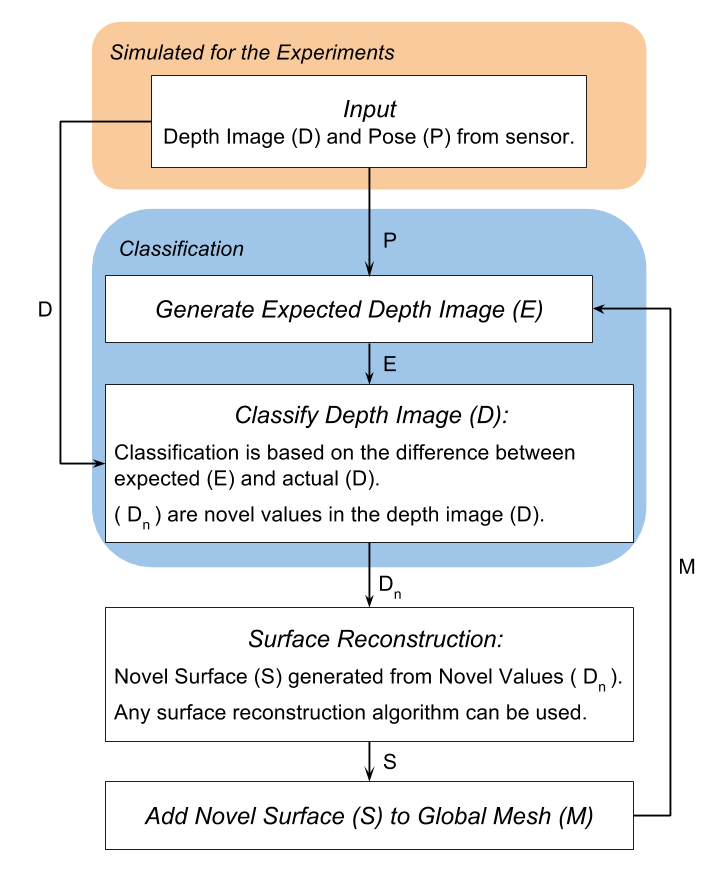
\includegraphics[width=.70\textwidth]{figures/diagram_system.png}
  \caption{MABDI system diagram}
  \label{fig:system}
\end{figure}

\begin{table}[h]
  \caption{Basic description of the main variables}
  \label{tab:var}
  \begin{center}
    \begin{tabular}{|c|l|}
    \hline
    {\bf Variable Name} & \multicolumn{1}{|c|}{{\bf Description}} \\
    \hline
    \rowcolor{LightGray} $D$ & Depth image from RGB-D sensor \\
    $P$ & Pose of the sensor \\
    \rowcolor{LightGray} $D_n$ & Parts of $D$ that are \emph{novel} \\
    $S$ & Novel surface generated from $D_n$ \\
    \rowcolor{LightGray} $M$ & Global mesh \\
    \hline
    \end{tabular}
  \end{center}
\end{table}

The system diagram is very similar to Fig. \ref{fig:pipeline} with the exception
of the Classification component, shown in blue. This Classification component is
MABDI's contribution to the state-of-art in mesh based mapping algorithms, and
is what gives MABDI the ability to make decisions about the incoming data. The
Classification component consists of two components:
\begin{enumerate}
    \item \textit{Generate Expected Depth Image $E$} - Here we take the global
    mesh $M$, render it using computer graphics, and use the depth buffer of the
    render window to create a depth image $E$ of what we expect to see from our
    sensor. This method requires the current pose $P$ of the actual sensor
    (simulated for our experiments).
    \item \textit{Classify Depth Image $D$} - Here we classify the actual depth
    image $D$ (simulated for our experiments) by first taking the absolute
    difference between $E$ and $D$ and thresholding. If the differences are
    small, those points are thrown away and if the differences are large, those
    points are kept as $D_n$. The idea behind this is, if the difference is
    large, the measurements are coming from a part of the environment that has
    not been seen before, i.e. novel. The implication of this assumption is that
    this version of MABDI cannot handle object removal. It is worth noting
    that MABDI can be extended to handle object removal by using the sign of the
    difference between $E$ and $D$ instead of the absolute value.
\end{enumerate}

% Simulated for the Experiments
The system diagram in Fig. \ref{fig:system} also shows the Input and the Surface
Reconstruction components. The Input component has been simulated for our
experiments. More details of this simulation will be covered in Chapter
\ref{chapter:experimental_setup}. The Surface Reconstruction component of the
MABDI algorithm can be implemented with any viable surface reconstruction
method. Our implementation utilizes the structural information contained within
the depth image. We will discuss this in more detail in the next section.

\section{Implementation}

\subsection{Surface Reconstruction}
\label{subsection:surface_reconstruction}

A depth image is not simply a set of unorganized points, but has inherent
structural information as well. This characteristic of the depth image allows us
to define a topology on the two dimensional depth image that is preserved when
projected to real-world coordinates. Our surface reconstruction method defines a
topology that is visualized in Fig. \ref{fig:srm}. Here elements of the mesh
are shown in light blue and novel points $D_n$ are shown as blue dots. The red
dot signifies a point that is not from the set $D_n$. Our implementation removes
all mesh elements that include such points, as seen in the figure.

\begin{figure}[h]%[thpb]
\centering
  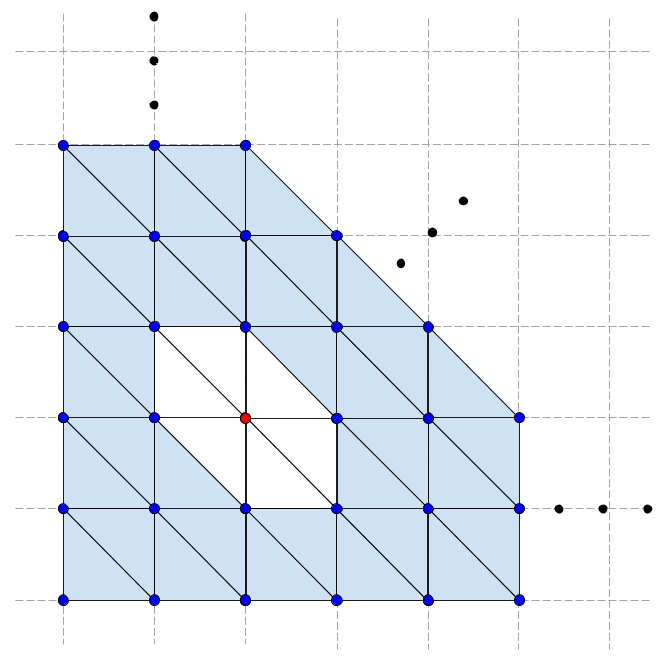
\includegraphics[width=.70\textwidth]
    {figures/diagram_surface_reconstruction.png}
  \caption{Topology defined on the depth image}
  \label{fig:srm}
\end{figure}

In order to remove elements defined by points that lie on completely different
surfaces, a step was added that uses imaging techniques in the form of a
convolution filter. A two dimensional, backward differencing convolution filter
is passed over the depth image. This filter has a magnified response at points
where the difference between neighboring pixels is large. Remembering pixel
values signify depth, it is assumed points with large differences between
themselves and their neighbor lie on different surfaces and so are marked as
invalid and all elements that use them are removed.

Our surface reconstruction method was chosen for its ability to be implemented
simply and run quickly. One consequence of our method is that the resulting
surface $S$ can have a large number of elements. For example, if all points from
$D$ are classified as novel (this happens on the first frame), $S$ can contain
over 600,000 elements. This assumes $D$ has no invalid points, e.g., out of the
sensor's range. Many surface reconstruction methods have been developed to
create a surface more intelligently, as discussed in Chapter
\ref{chapter:related_works}. For example, the advancing front method developed
by Marton et al. \cite{Marton2009} is capable of creating surfaces with fewer
elements than our method by utilizing a robust resampling method. One great
thing about the MABDI algorithm is that the method developed by Marton et al.
can be used in place of our surface reconstruction method. This characteristic
of MABDI is great because MABDI does not depend on the choice of surface
reconstruction method and the method can be chosen as the state-of-the-art
changes or to suit a particular application. Also, due to our implementation's
modular software design, the entire code base would not need to be changed in
order to accomplish this. We will discuss the software design in the next
section.

\subsection{Software Design}

From a software perspective, the major difficulty of implementing the MABDI
algorithm was found to be creating both the simulated depth image $D$ and the
expected depth image $E$. In addition, managing the complexity of the data
pipeline needed to run the algorithm and the simulation of the sensor proved to
be difficult. Thankfully, Kitware, which is a leading edge developer of
open-source software, created the Visualization Toolkit (VTK)
\cite{schroeder2004visualization, sitevtk}. At the time of this writing the VTK
Github repository has over 60,000 commits and is contributed to by supporters
such as Sandia National Labs \cite{sitesandia}.

VTK is suitable for the implementation of MABDI for many reasons. Perhaps
the most important is the concept of a vtkAlgorithm (often called a Filter).
This allows a programmer to create a custom and modular processing pipeline by
defining classes that inherit vtkAlgorithm and then defining the connections
between these classes. For example, you could have a pipeline that reads an
image from a source (component 1), performs edge detection (component 2), and
then renders the image (component 3).

Using the concept of VTK filters, the individual elements of MABDI can be
succinctly defined in individual classes. With that in mind, we can see in Fig.
\ref{fig:software} the layout used in our implementation of MABDI. vtkImageData
and vtkPolyData are VTK types used to represent an image and mesh respectively.
The elements shown in blue in Fig. \ref{fig:software} are the core components of
the MABDI algorithm and are implemented as custom VTK filters. Their source code
is included in Appendix \ref{appendix:mabdi_code}. Here we will discuss all
components in detail:

\begin{sloppypar}
\begin{itemize}
    \item  \textit{Source} - Classes with the prefix Source define the
    environment that is used for the simulation and provide a mesh in the form
    of a vtkPolyData.
    \item \textit{FilterDepthImage} - Render the incoming vtkPolyData in a
    window and output the depth buffer from the window as a vtkImageData. The
    output additionally has pose information of the sensor.
    \item \textit{FilterClassifier} - Implements the true innovation of MABDI,
    i.e., takes the difference between the two incoming depth images
    (vtkImageData) and outputs a new depth image where the data that is not
    novel is marked to be thrown away.
    \item \textit{FilterDepthImageToSurface} - Performs surface reconstruction
    on the novel points. For more detail see Section
    \ref{subsection:surface_reconstruction}. The surface is output as a
    vtkPolyData.
    \item \textit{FilterWorldMesh} - Here we simply append the incoming novel
    surface to a growing global mesh that is also output as a vtkPolyData.
\end{itemize}
\end{sloppypar}

\begin{figure}[b]%[thpb]
\centering
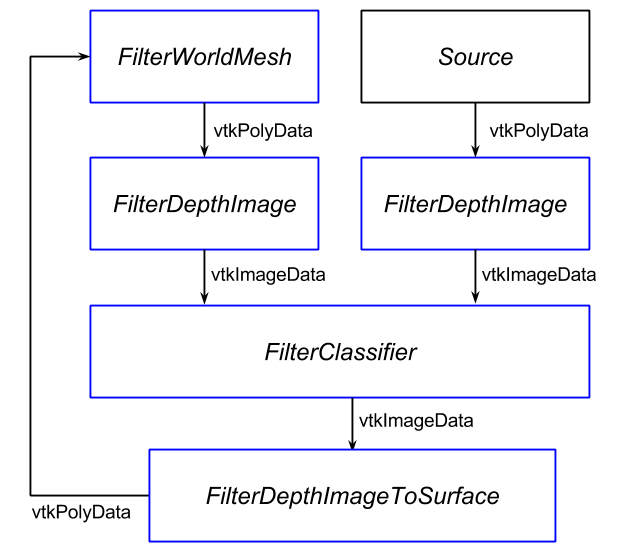
\includegraphics[width=.75\textwidth]{figures/diagram_software.png}
\caption{MABDI software diagram}
\label{fig:software}
\end{figure}

MABDI is implemented in Python and uses VTK. Our implementation is distributed
under the BSD license and is available on Github at the address below:

$$
https://github.com/lucasplus/MABDI
$$

At the time of this writing, it consists of over 1,400 lines. The code that
implements the MABDI algorithm itself is around 750 lines.

% How Mabdi works, describe the algorithm
% How Mabdi is implemented

\chapter{Experimental Setup}	\label{chapter:experimentalsetup}

It was decided to develop and test MABDI in a completely simulated environment
so that all results could be repeatable and also to facilitate the ability to
debug during the development process. This ability was truly invaluable as some
components of the algorithm proved to be complex from an implementation
perspective. In addition, we can now compare the resultant
global mesh to ground truth.

\section{Simulation Parameters} \label{chapter:experimentalsetup:simulationparameters}

The simulation was designed to be highly configurable and is implemented by a
class named MabdiSimulate. The class is initialized with parameters that control
all aspects of the simulation. Parameters of a particular importance are
discussed in more detail here:

\begin{itemize}
    \item  Environment - This parameter specifies the environment used to generate
    the simulated depth images. \textit{Table} is an environment consisting of a
    table and two cups placed on the table. The table is 1 meter tall.
    \textit{Bunnies} is an environment consisting of three bunnies who are
    around 1.5 meters tall. These bunnies are created using the Stanford Bunny
    \cite{Turk1994}, a well known data set in computer graphics.
    \item Noise - If true, adds noise to the depth image of the simulated sensor.
    \item Dynamic - If true, adds an object during the simulation. In the case
    of this analysis, a third bunny is added half-way through the simulation.
    \item Iterations - The number of iterations the simulation will have. This
    parameter affects the distance the sensor travels from frame to frame.
\end{itemize}

% parameters chosen the experimental runs
For this paper we will be exploring three experimental runs to demonstrate the
ability of the MABDI implementation to generate valid results. Additionally, the
experimental runs will be able to show the capabilities of the MABDI algorithm
such as handling object addition in the environment.

\begin{table}[h]
  \caption{Description of the experimental runs.}
  \label{tab:run}
  \begin{footnotesize}
  \begin{center}
    \begin{tabular}{|l|c|c|c|c|}
    \hline
           & Environment & Noise   & Dynamic & Iterations \\\hline
    Run 1	 & Table       & False   & False   & 30 \\
    Run 2  & Bunnies     & True    & False   & 50 \\
    Run 3  & Bunnies     & True    & True    & 50 \\
    \hline
    \end{tabular}
  \end{center}
  \end{footnotesize}
\end{table}

All experimental runs define a helical path for the sensor to follow during the
simulation. The path circles the objects in the environment twice. A helical
path was chosen because it returns to a part of the environment that has been
already mapped and is thus ``known'' to the global mesh. Also, because the path
is a helix and not just a circle, the sensor views the environment from a
slightly different position on each pass.

\section{Analysis of Simulated Noise} \label{chapter:experimentalsetup:analysisofsimulatednoise}

In order to realistically simulate the sensor in a real-world environment we add
noise to the depth image $D$. See Fig. \ref{fig:system}. The magnitude of the
noise added is based on the accuracy of real-world sensors. As new RGB-D sensors
have been developed, such as the Asus Xtion and the Kinect for Xbox One, the
accuracy of the sensors has continued to improve \cite{lachat2015first}. For
this work, we take a conservative approach and utilize the well known error
modeling work of Khoshelham \cite{Khoshelham2012} that is based on the original
Kinect.

The depth image used by the MABDI algorithm $E$ and the depth image that comes
from simulating the environment $D$ both use a pinhole camera model. This method
has been validated in the localization work of Fallon \cite{Fallon2012}. The
intrinsic camera parameters of the pinhole hole model were chosen to emulate the
Kinect sensor \cite{sitekinectspecs}. The pinhole model defines a transformation
matrix used to transform between viewpoint coordinates and real-world
coordinates. The z component of the viewpoint coordinates constitutes the depth
image and are defined to vary between 0 and 1. Due to how the transformation
works, differences in the depth image do not linearly correspond to changes in
real-world coordinates as can be seen in Fig. \ref{fig:depth}.

\begin{figure}[h]%[thpb]
\centering
  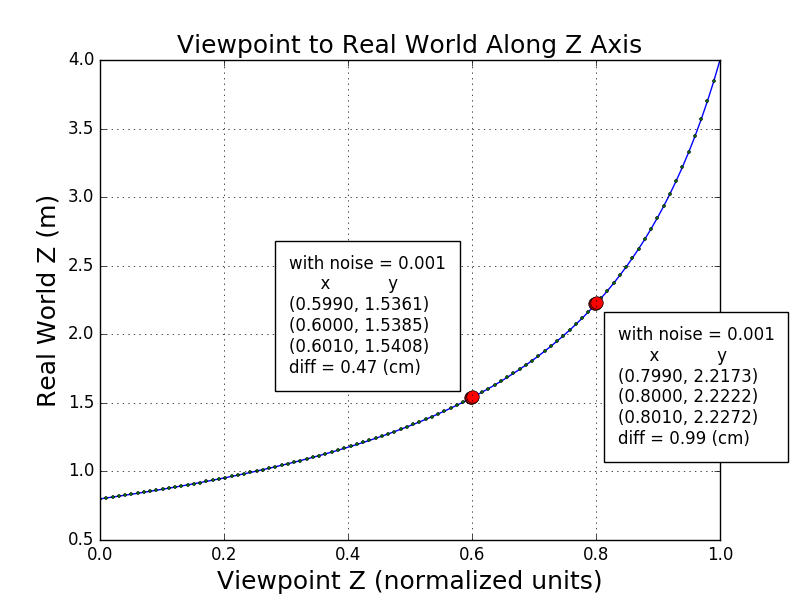
\includegraphics[width=.75\textwidth]{figures/plot_depth.png}
  \caption{Viewpoint coordinates to real world coordinates analysis.}
  \label{fig:depth}
\end{figure}

The noise added to $D$ is defined by the equation below. The standard deviation
$\sigma\mathsmaller{=}0.001$ was chosen so that the resultant errors in the
real-world coordinates would correlate to the error model in
\cite{Khoshelham2012}. The text boxes in Fig. \ref{fig:depth} show the resultant
real-world error for two values of $D$; they match the error model of
\cite{Khoshelham2012}.

$$
D_{noisy}(i,j) = D(i,j) + D(i,j)*\mathcal{N} (\mu\mathsmaller{=}0, \sigma\mathsmaller{=}0.001)
$$

% Viewpoint coordinates to real-world coordinates analysis. Viewpoint coordinates
% are obtained when a mesh is rendered into a render window, and can be
% transformed to real-world coordinates using the transformation matrix of the
% camera. Noise is added in simulation to the viewpoint coordinates. This graph
% shows the effect of that noise in real-world coordinates.

% describe the simulation environment
% maybe determine speed of walker
% discuss noise

\chapter{Results} \label{chapter:results}

% overview of runs
% explanation of the dashboard view
% dashboard results
% resultant mesh results

For each experimental run, a dashboard view was created that can be shown for
each iteration of the simulation. The dashboard view combines several different
views of information useful for understanding the inner workings of the MABDI
algorithm. As an example, Figure \ref{fig:run1} shows the dashboard view for the
first experimental run. For these experiments, all dashboard views follow the
same pattern as described below:

\begin{itemize}
  \item (a) - Shows the global mesh $M$ from a third-person point of view and in
  the context of the simulated environment. The multi-colored mesh is $M$. The
  mesh is multi-colored in order to show the passage of time. For example, in
  Run1, The mesh is colored yellow, light green, and dark green for iterations
  1, 2, and 3 respectively. Additional items in the view show elements of the
  simulated environment: the wire frame corresponds to the viewing frustum of
  the sensor, the light blue helical line is the path of the sensor, and the
  translucent gray mesh is the simulated environment.
  \item (b) - Same as (a) except it shows the novel surface $S$ instead of
  the global mesh $M$.
  \item (c) - Plot showing the number of elements in the global mesh $M$
  after this iteration.
  \item (d \& e) - Actual $D$ and expected $E$ depth image
  respectively.
  \item (f) - The classified depth image. Points that will be used to generate
  the novel surface $S$ are shown in black. Points to be thrown away are shown
  in white.
\end{itemize}

The dashboard views are an excellent way to visualize important aspects of
MABDI. In the next section, Section \ref{section:results1}, we will utilize key
dashboard views to look at the behavior and performance of MABDI at one particular iteration of each experimental run. In section \ref{section:results2} we will analyze the
quality and progression of the resultant global mesh from each experiment.

\section{MABDI Performance During Experiments}
\label{section:results1}

\subsection{Experiment 1}

Figure \ref{fig:run1} shows the dashboard view of the first experiment during
the third iteration. Note that \ref{fig:run1}(a) shows $M$ after the third
iteration. As stated before, $M$ is multi-colored in order to show the passage
of time. The mesh is colored yellow, light green, and dark green for iterations
1, 2, and 3 respectively. \emph{During iteration 3, $M$ is composed of only the
yellow and light green parts.}

\begin{figure}[h]%[thpb]
\centering
  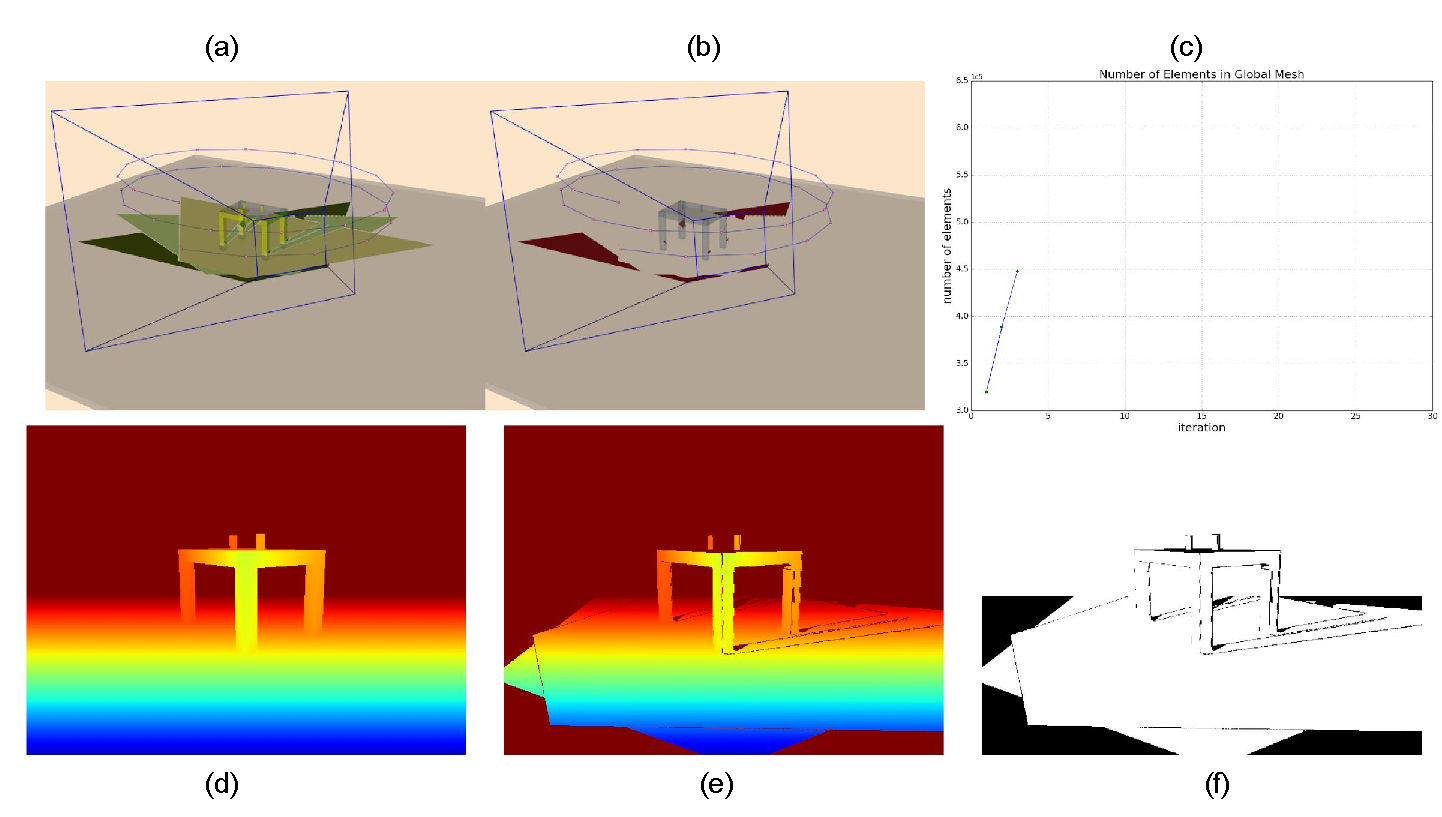
\includegraphics[width=\textwidth]{figures/diagram_run1.pdf}
  \caption{Dashboard view of the first experimental run.}
  \label{fig:run1}
\end{figure}

Examining Figure \ref{fig:run1} demonstrates how the novel surface
$S$ is appended to the global mesh $M$ after each iteration of MABDI. Let's use
the figure to follow the process. It will be useful to refer to Figure
\ref{fig:system} for this section.

\begin{sloppypar} % to get rid of weird black box thing
\begin{enumerate}
  \item Input - \ref{fig:run1}(d) shows the depth image $D$ generated from the
  simulated sensor. \ref{fig:run1}(a) shows us two important aspects to consider
  about $D$. First, the pose $P$ of the sensor is shown by looking at the
  sensor's view frustum, indicated by the blue wireframe. Second, the only
  environmental information used to generate the depth image is shown in light
  gray.
  \item Generate Expected Depth Image ($E$) - \ref{fig:run1}(e) shows the
  expected depth image $E$. \ref{fig:run1}(a) also shows us two important
  aspects to consider about $E$. First, the same pose $P$ is used to create both
  $D$ and $E$ (as indicated by the blue wire frame). Second, the only
  environmental information used to create $E$ is the yellow and light green
  parts of $M$ because that is the only information $M$ contains \emph{during}
  iteration 3.
  \item Classify Depth Image ($D$) - \ref{fig:run1}(f) visualizes the
  classification process. More specifically, it shows the points as expressed in
  Equation \ref{eqn:throwaway} in white ($D_{throwaway}$). \ref{fig:run1}(f) is
  important for understanding how MABDI works because it clearly shows which
  points will be thrown away (white) and which points will be kept for
  generating the novel surface $S$ (black).
  \item Surface Reconstruction - \ref{fig:run1}(b) shows the novel surface $S$
  in the context of the simulated environment. $S$ is constructed using all the
  points colored black in \ref{fig:run1}(f).
  \item Add Novel Surface ($S$) to Global Mesh($M$) - \ref{fig:run1}(a) shows
  the novel surface $S$ appended to the global mesh $M$ in dark green.
\end{enumerate}
\end{sloppypar}

\subsection{Experiment 2}

The second experiment gives us a clear example of how the classification process
is able to identify points from the depth image $D$ that correspond to parts of
the environment that have not been seen before. In this example the global mesh
$M$ has a partial representation of the objects in the environment and when the
sensor is moved to the next pose $P$, the new perspective reveals a portion of
the object that has not been seen before. This \emph{novel portion} of the
environment, which we will be referring to, is shown by the red ellipse in Figure
\ref{fig:run2_novel_portion}.

\begin{figure}[h]%[thpb]
\centering
  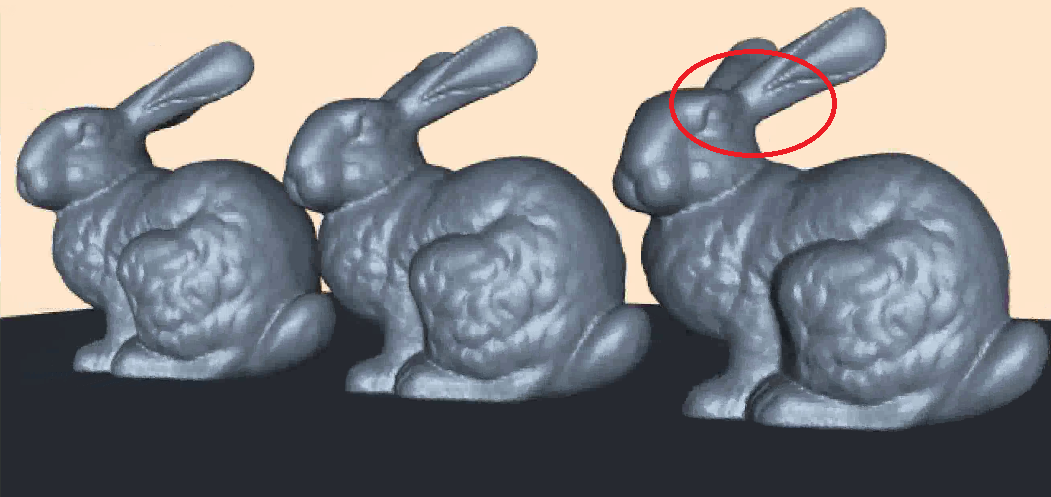
\includegraphics[width=0.8\textwidth]{figures/run2_novel_portion.png}
  \caption{\emph{Novel portion} of the environment that we will be referring to
  in this section.}
  \label{fig:run2_novel_portion}
\end{figure}

Figure \ref{fig:run2} shows the dashboard view of the second experiment during
the second iteration. Using the dashboard view, we can follow how MABDI handles
the novel portion of the object step-by-step:
\begin{enumerate}
  \item \ref{fig:run2}(a) shows the global mesh $M$. The yellow portion of the
  mesh constitutes the entirety of $M$ after the first iteration. We can see the
  novel portion of the environment was not represented in $M$ after the first
  iteration due to occlusion.
  \item \ref{fig:run2}(d) shows the depth image $D$ from the new sensor pose
  $P$. We can see the novel portion can be seen by the sensor on this iteration.
  \item \ref{fig:run2}(e) shows the expected depth image $E$. During the second
  iteration $M$ consists of only the yellow portion shown in \ref{fig:run2}(a)
  consequently, $E$ does not show any points in the area corresponding to the
  novel portion of the environment.
  \item \ref{fig:run2}(f) shows the classification process successfully
  identifying points in $D$ that correspond to the novel portion as indeed
  novel. In the figure the points are highlighted by a red circle.
  \item \ref{fig:run2}(b) shows the novel surface $S$ now represents the novel
  portion of the environment.
  \item Finally, the orange mesh in \ref{fig:run2}(a) shows the novel portion of
  the environment is now represented by the global mesh $M$.
\end{enumerate}

\begin{figure}[h]%[thpb]
\centering
  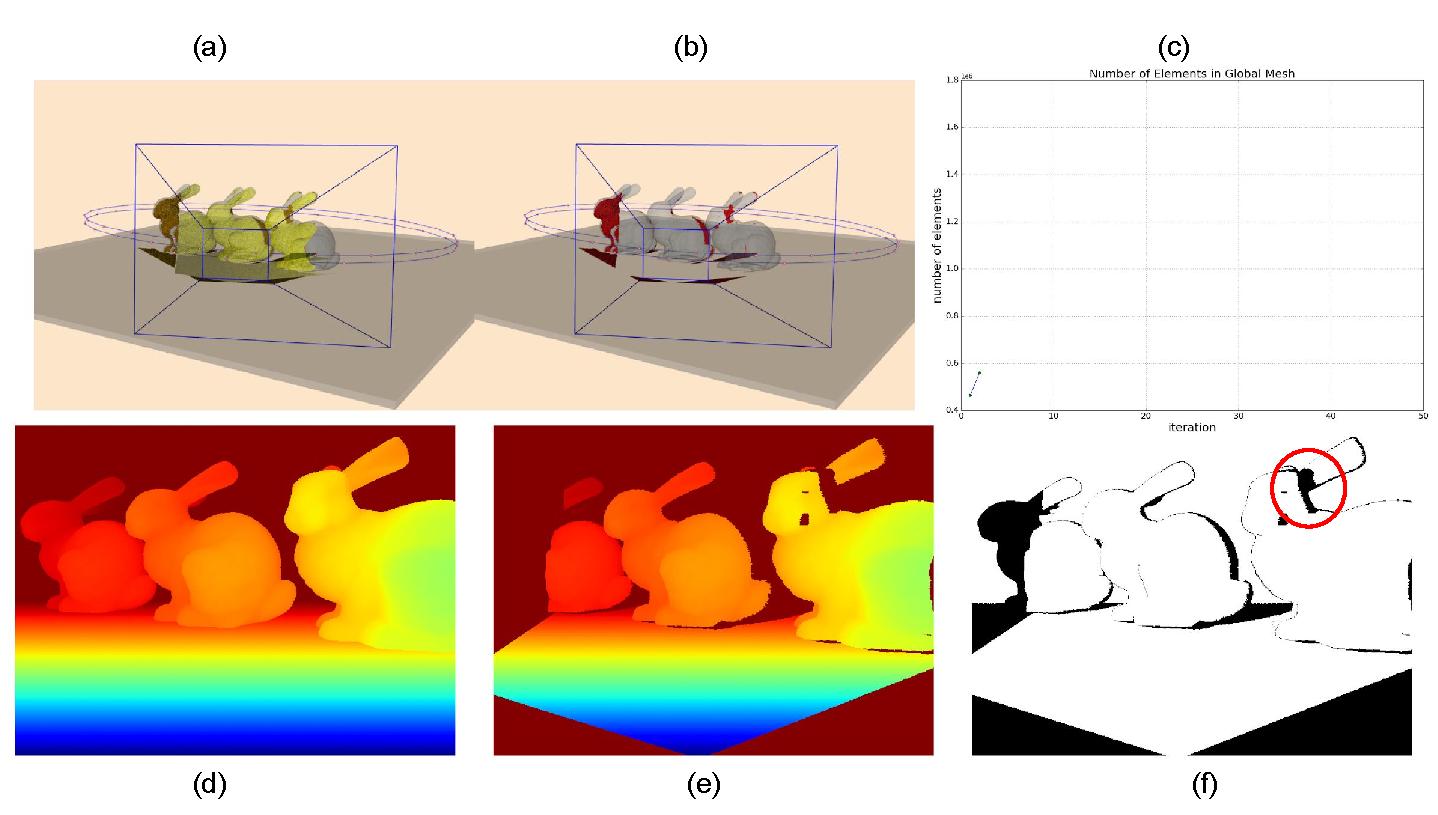
\includegraphics[width=\textwidth]{figures/diagram_run2.pdf}
  \caption{Dashboard view of the second experimental run.}
  \label{fig:run2}
\end{figure}

\subsection{Experiment 3}

Experiment three shows how MABDI reacts to object addition. Figure
\ref{fig:run3} shows the dashboard view of the third experiment during the
twenty-sixth iteration. At this iteration the middle bunny is suddenly added to
the simulated environment. We can use the dashboard view to see the behavior of
MABDI to this new object:
\begin{enumerate}
  \item In \ref{fig:run3}(d) we see the depth image $D$ shows the new bunny.
  \item In \ref{fig:run3}(e) the expected depth image $E$ does not show the new
  bunny because $M$ has no representation of the new bunny.
  \item \ref{fig:run3}(f) shows the classification process successfully
  identified the points corresponding to the new bunny as novel.
  \item The novel points are used to generate the novel surface $S$ and then $S$
  is appended to $M$, shown in \ref{fig:run3}(a \& b).
  \item The addition of the new object resulted in a $S$ with a large number of
  elements for this particular iteration. \ref{fig:run3}(f) plots the resulting
  jump in the number of elements contained with $M$.
\end{enumerate}

\begin{figure}[h]%[thpb]
\centering
  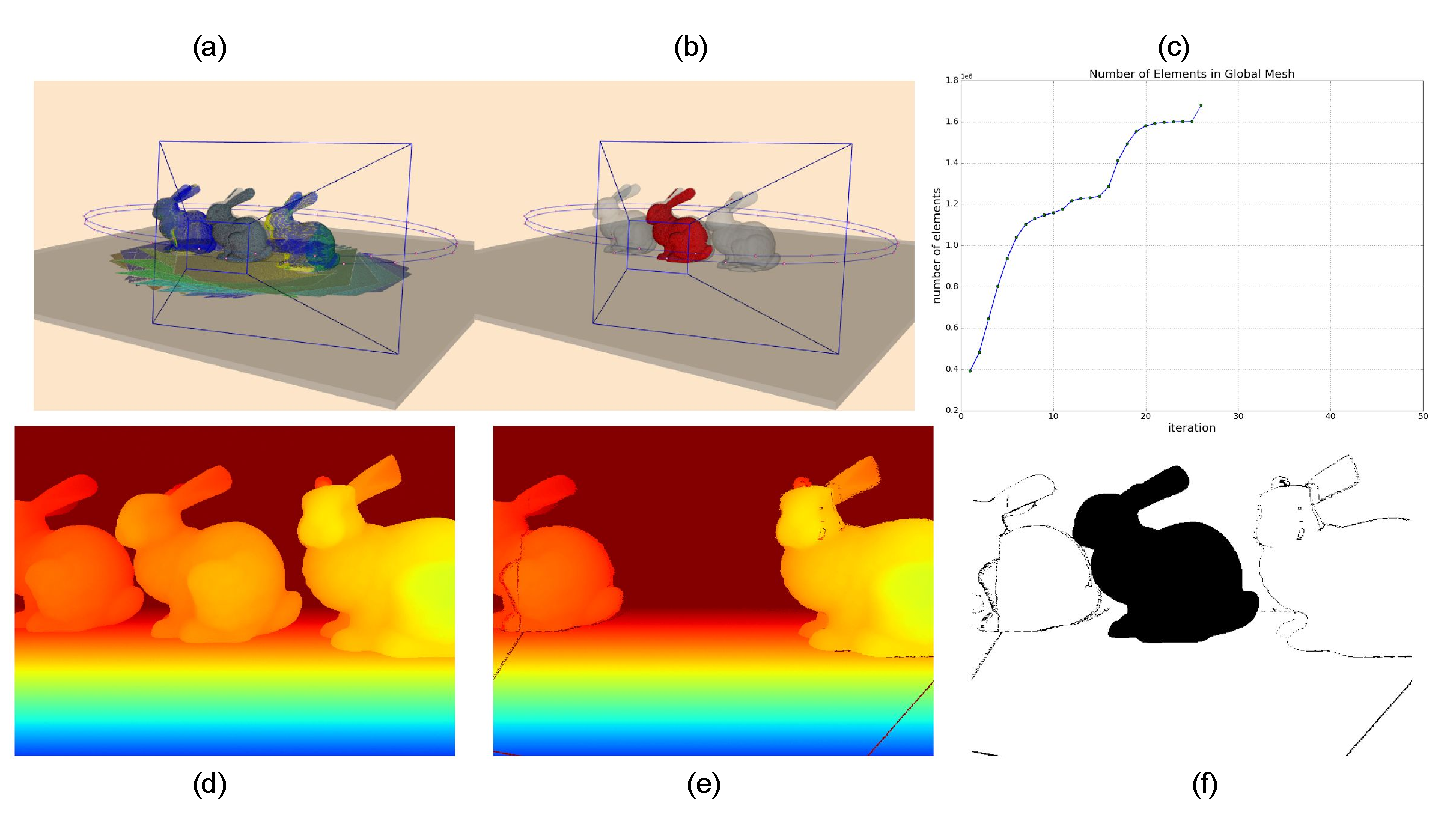
\includegraphics[width=\textwidth]{figures/diagram_run3.pdf}
  \caption{Dashboard view of the third experimental run.}
  \label{fig:run3}
\end{figure}

\section{Global Mesh Results}
\label{section:results2}

\subsection{Mesh Quality}

% quality of the mesh
Figure \ref{fig:gm_3_full} shows the resultant global mesh from experiment 3. In
this section we will use this figure to make observations about the quality of
the global mesh for all three experiments.

There are gaps in the mesh that occur typically along the boundaries
of where the novel surface $S$ is appended to the global mesh $M$. This behavior
is common for Surface Reconstruction methods as those discussed in Section
\ref{section:surface_reconstruction}. Algorithms exist for merging these gaps as
a post processing step such as Turk's Zippered Polygon Meshes \cite{Turk1994}.
The aforementioned methods are typical for single object reconstruction.
Traditional mesh-based environmental mapping algorithms simply append
overlapping layers of mesh resulting in no gaps but a heavily redundant
representation with a high memory cost.

The mesh is noisy. This noisiness is due to the simplicity of our
implementation's surface reconstruction method as discussed in Section
\ref{subsection:surface_reconstruction}. Our method simply connects neighboring
points in the point cloud without additional steps such as Laplacian smoothing
\cite{Nealen2006}. Our reconstruction method was sufficient for
demonstrating the usefulness of the MABDI algorithm, but results in a mesh with
the same magnitude of noise as the sensor's simulated noise.

\begin{figure}[h]%[thpb]
\centering
  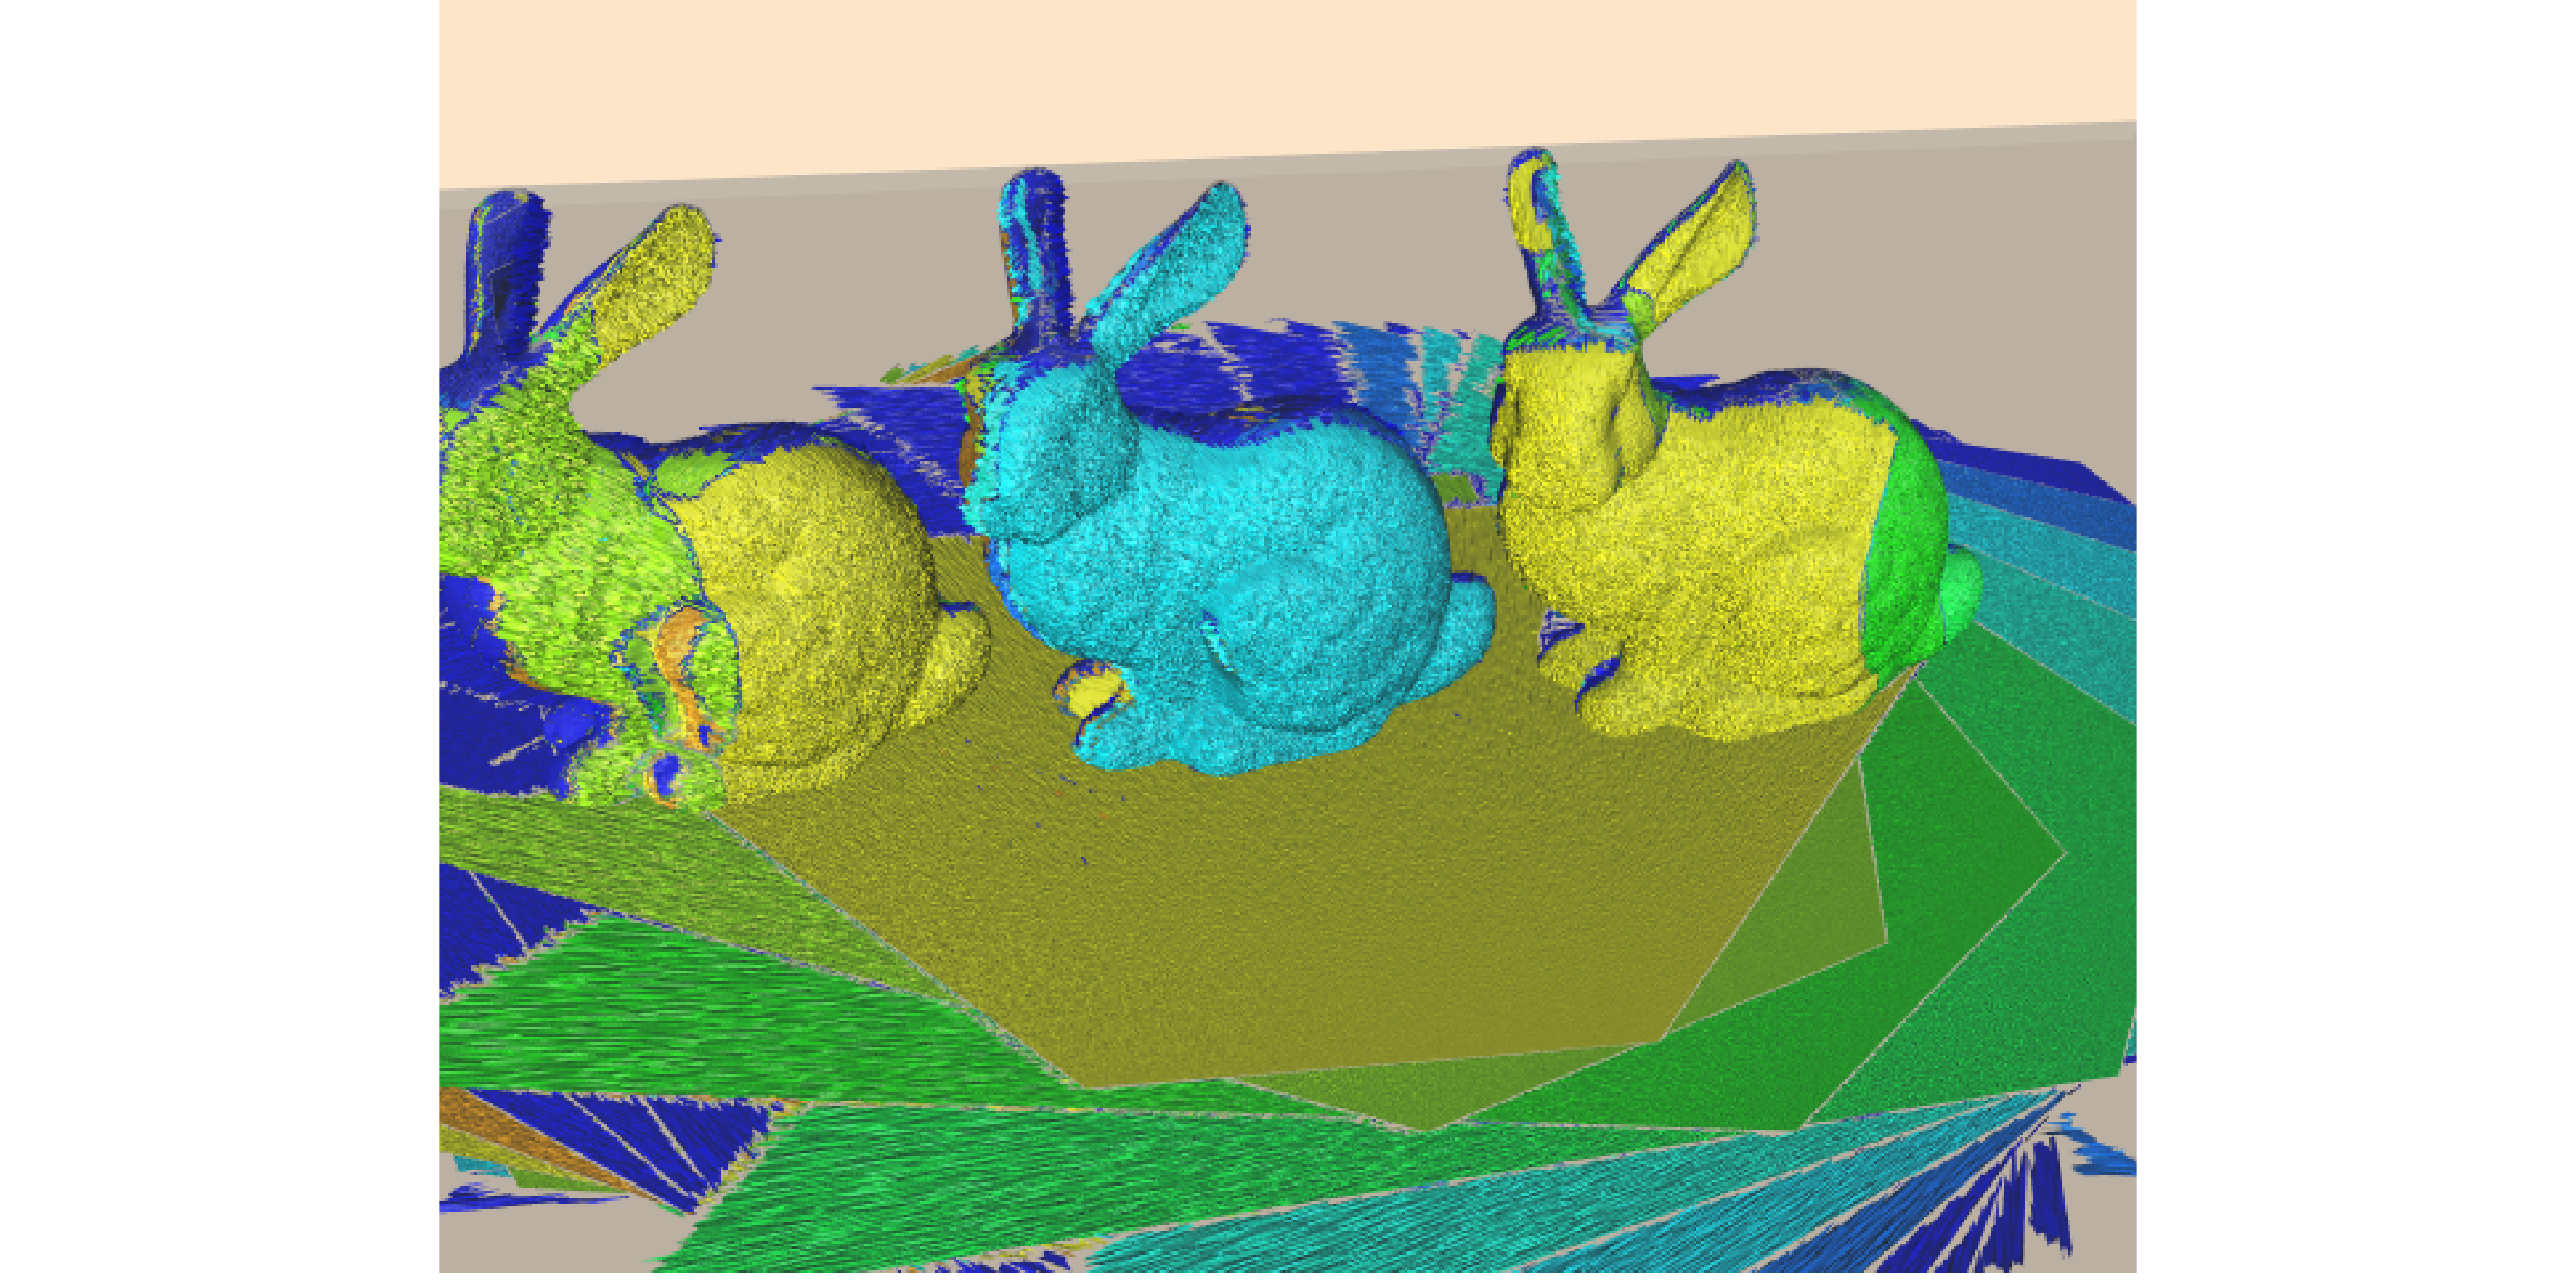
\includegraphics[width=\textwidth]{figures/run3_global_mesh.png}
  \caption{Global mesh at the end of experiment 3.}
  \label{fig:gm_3_full}
\end{figure}

\subsection{Mesh Progression}

% shape of the graphs
To appreciate the true benefit of the MABDI algorithm it is helpful to look at
how the number of elements in the global mesh $M$ progress over time. In this
section we will analyze plots showing how the number of elements in $M$ change
during the experiments. Note, the dashboard views also showed this plot. For
example, the plot of Figure \ref{fig:gm_1} is the same as Figure
\ref{fig:run1}(c), but Figure \ref{fig:gm_1} shows the plot at the completion of
the experiment.

Figure \ref{fig:gm_1} shows the resultant mesh and mesh progression for the
first experiment. The plot highlights the major difference between MABDI
and traditional mesh-based environmental mapping methods. Traditional methods
would have a plot similar to that indicated by the red arrow on the graph
because these methods have no ability to identify or remove redundant mesh
elements. Due to MABDI's algorithmic design, MABDI has the intrinsic ability to
identify points in the depth image corresponding to parts of the environment
that are already known by the global mesh $M$. MABDI then simply does not use
those points for surface reconstruction and consequently does not create
redundant mesh elements. For this reason, the number of elements in $M$ levels
off as the environment becomes more known.

\begin{figure}[h]%[thpb]
\centering
  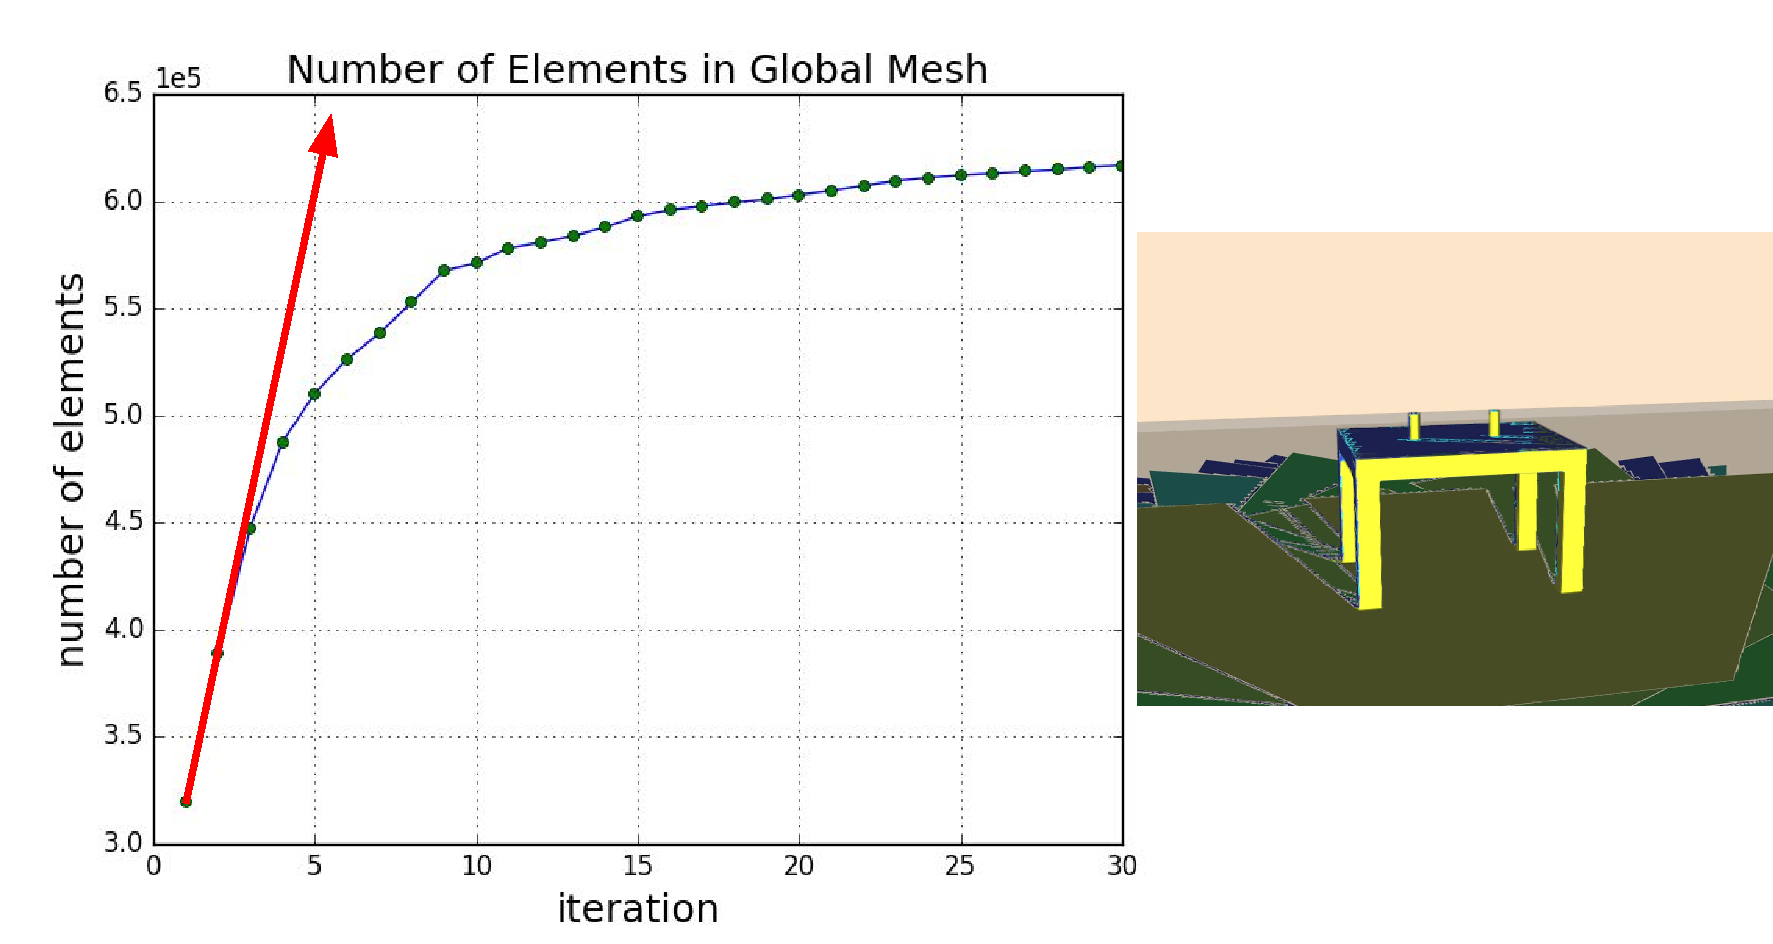
\includegraphics[width=\textwidth]{figures/diagram_run1_gm.pdf}
  \caption{Experiment 1 global mesh results.}
  \label{fig:gm_1}
\end{figure}

Figure \ref{fig:gm_2} shows us the resultant mesh after the second experiment.
Here we can see that MABDI is reactive to the environment. In the preceding
experiment, the environment was symmetrical. In this experiment, the environment
is not symmetrical and we can see the effects by looking at the progression of
the global mesh $M$. First let us note that the sensor circles the objects twice
during the experiment and in total travels $720^{\circ}$ during the 50
iterations. We notice when the sensor gets to $90^{\circ}$ (around iteration
7) the number of elements begins to level off and then increases again as the
sensor travel to $270^{\circ}$ (around iteration 19). This behavior occurs
because the information rich perspectives of the environment occur at
$0^{\circ}$ and $180^{\circ}$. There is less for the sensor to look at when
viewing the environment from the sides. In this way, MABDI is reactive as the
sensor moves to parts of the environment that are rich in information.
Consequently, the mesh grows rapidly based on the needs of the environment.

\begin{figure}[h]%[thpb]
\centering
  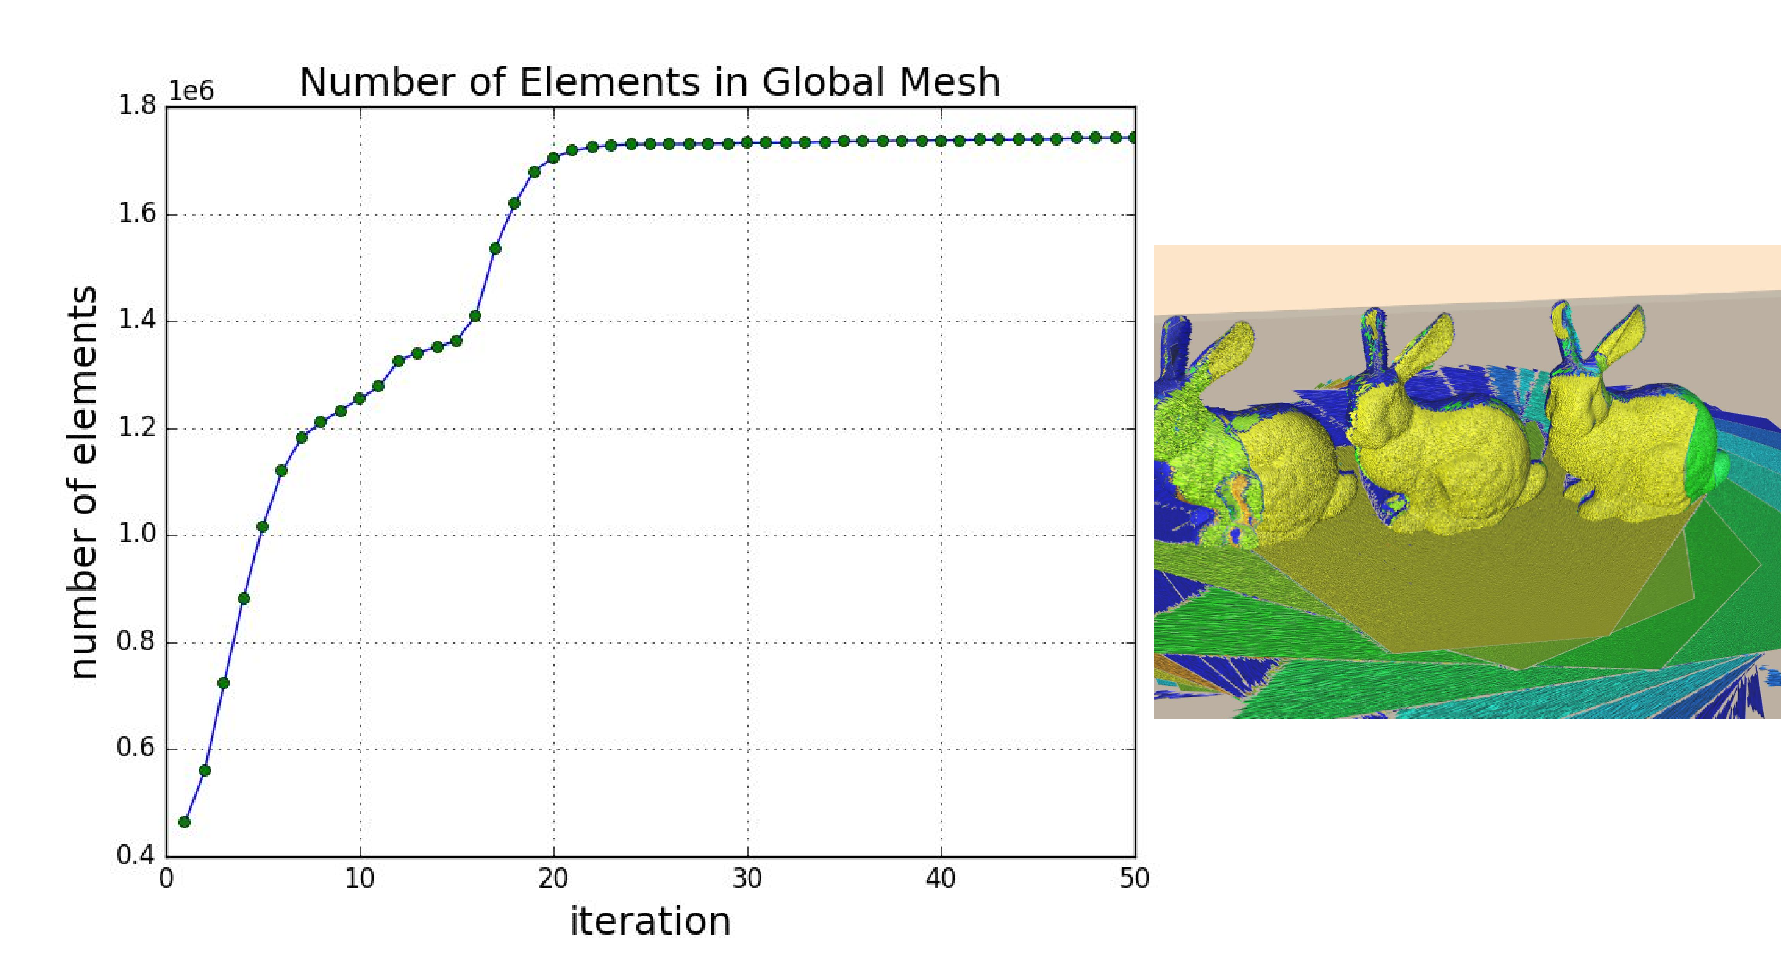
\includegraphics[width=\textwidth]{figures/diagram_run2_gm.pdf}
  \caption{Experiment 2 global mesh results.}
  \label{fig:gm_2}
\end{figure}

Figure \ref{fig:gm_3} shows us the resultant mesh after the third experiment. In
this experiment the middle bunny was added during the twenty-sixth iteration.
This object addition had two effects on the global mesh. First, it created a
sudden jump in the plot as highlighted by the red circle. Second, the middle
bunny is colored blue in the resultant mesh, signifying that it was added to $M$
during a different iteration than the bunnies on the left and the right. Both of
these effects indicate that MABDI was able to successfully identify the new
bunny as novel and incorporate the bunny in to the global mesh within one
iteration.

\begin{figure}[h]%[thpb]
\centering
  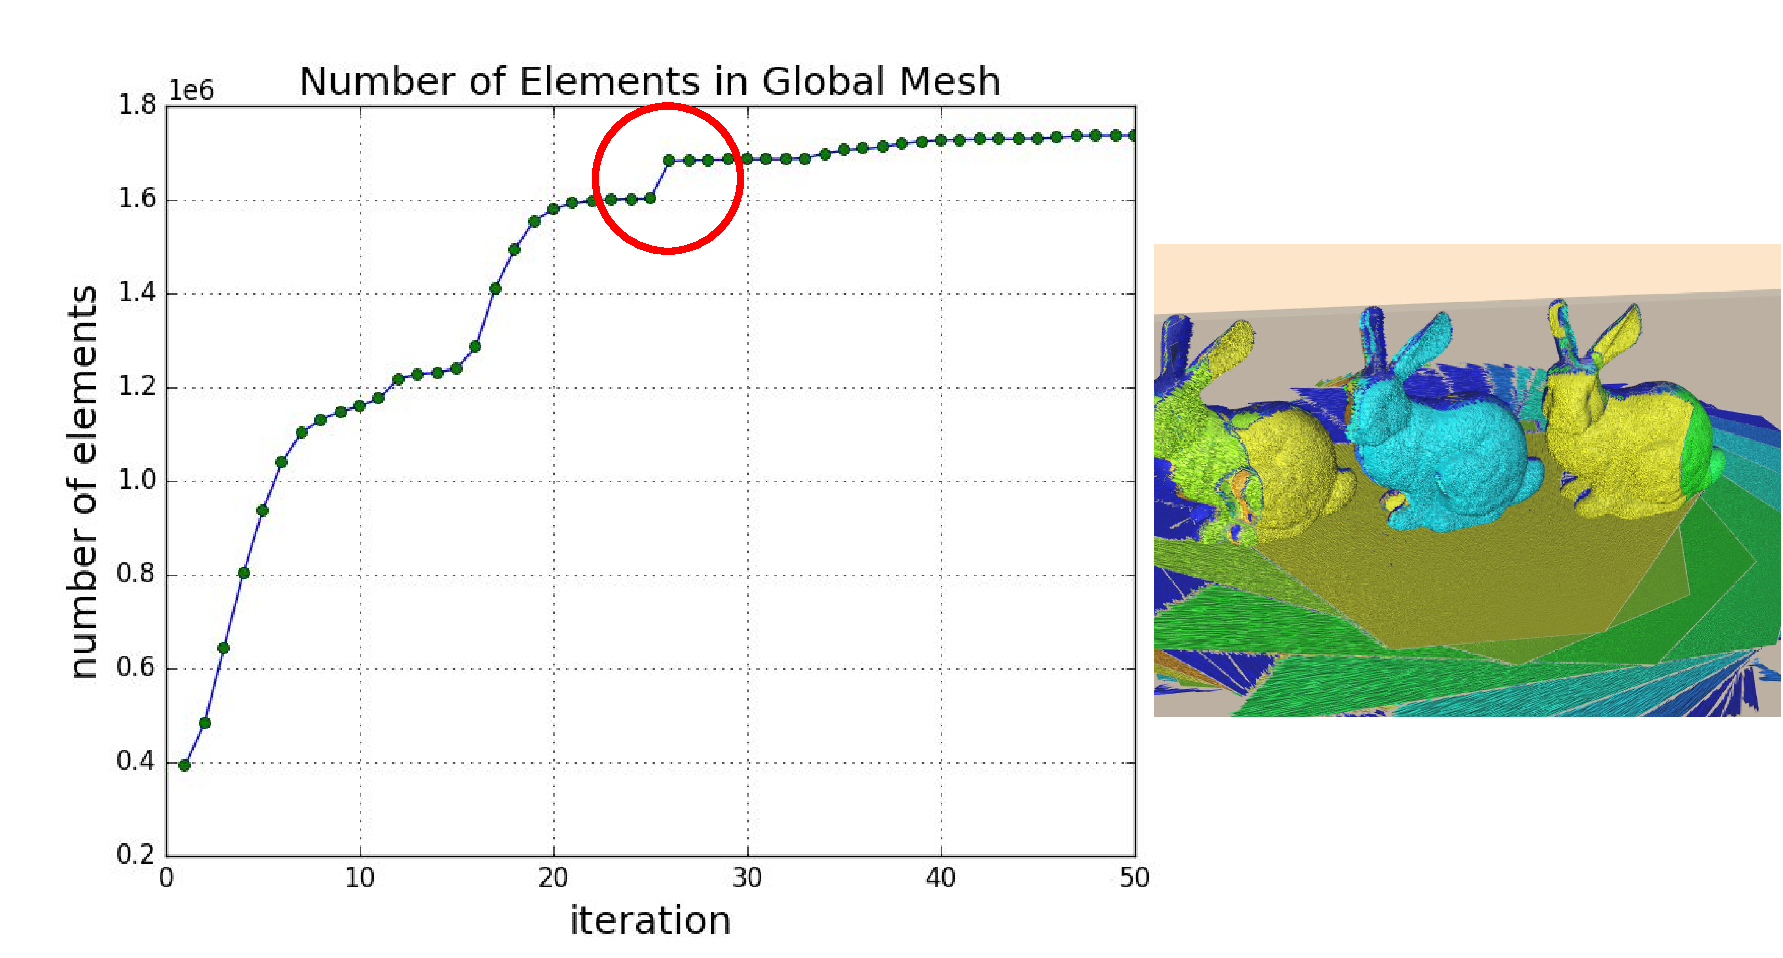
\includegraphics[width=\textwidth]{figures/diagram_run3_gm.pdf}
  \caption{Experiment 3 global mesh results.}
  \label{fig:gm_3}
\end{figure}

% Figure \ref{fig:gm} shows the resultant global mesh $M$ for each of the experiments
% along with a plot of the number of elements in the mesh over iterations. These
% plots show the main contribution of MABDI because they level-off as the
% environment becomes more known as opposed to traditional reconstruction methods
% where the number of elements increases linearly over time.

% Results of the runs
% Definitely talk about how adding a bunny worked well

\chapter{Conclusion} \label{chapter:conclusion}

The goal of MABDI is to determine data from the sensor that has not yet been
represented in the map and use this data to add to the map. MABDI does this by
leveraging the difference between what we are actually seeing and what we expect
to see. MABDI can work in conjunction with any current mesh-based surface
reconstruction algorithms, and can be thought of as a general means to provide
introspection to those types of reconstruction methods.

 The MABDI implementation was able to successfully perform in a realistic
 simulation environment. The results show how novel sensor data was
 successfully classified and used to add to the global mesh. Also, the MABDI
 algorithm runs at around 2Hz on a consumer grade laptop with an Intel i7
 processor. This performance means that it is capable of real-world
 applications.

 Currently MABDI is only designed to handle object addition, but the idea can be
 extended to handle both object addition and removal as discussed in Section
 \ref{section:algorithmic_design}. This would give the system the
 capability to handle highly dynamic environments such as a door opening and
 closing.

% discuss difficulty with noise
% how to expand to deal with object deletion

\bibliographystyle{IEEEtran}
\bibliography{bibliography}

\end{document}
